\documentclass[edit,11pt,ChapStyle3,twoside,doubleinterligne]{ManuscriptThese}

%%%%%%%%%%%%%%%%%%%
\usepackage{ParStartThese}
\usepackage{FontsThese}
\usepackage{UtilsThese}

\usepackage{eurofont} 	%used to generate the € symbol
%%%%%%%%%%%%%%%%%%%
\usepackage[french, english]{babel}
\usepackage[pdftex]{graphicx}

\usepackage{float}
\usepackage{url}
\usepackage{makeidx}

\usepackage[T1]{fontenc}

\usepackage{amsmath, amsthm, amssymb}	%draw nice maths

\usepackage{hyperref} %for urls

%where to find the figures
\graphicspath{ {figs/} {StateoftheArt/figs/} {MAS4Optim/figs/} }

%%%%%%%%%%%%%%%%%%%
% custom commands

%Insert a definition =>  \defintion{title}{content}
\newcommand{\definition}[2]{
   \begin{quotation}	\parbox{0.9\textwidth}
		{\textbf{Definition -  #1: }#2}
  \end{quotation} 
} 

%%%%%%%%%%%%%%%%%%%
%%%%%%%%%%%%%%%%%%%
%%%%%%%%%%%%%%%%%%%

\makeindex
\author{\@ThesisAuthorFirstName \@ThesisAuthorLastName}
\title{\@ThesisTitle}

\begin{document}

%-------------------------------------------------------------------
%                         Page de titre:
%-------------------------------------------------------------------
% La page de titre se compose automatiquement avec la commande
% \MakeThesisTitlePage
% Certains champs ont des valeurs par d\'efaut (Th\`ese pr\'esent\'ee \`a...),
% valeur qui d\'epende du style utilis\'e (rennes1, ou brest)
%
% l'exemple suivant fait le tour des commandes modifiables

%\newcommand{\MakeThesisSynthesisPage}%
%{%
%  \newpage
%  \@cover@hook
%  \thispagestyle{empty}
%  \begin{changemargin}{-1.5cm}{-1cm}
%    \thesissynthesispgebody
%  \end{changemargin}
%  \newpage  
%  \if@twoside
%  \thispagestyle{empty}
%  \hbox{}
%  \par\vfill
%  \newpage
%  \addtocounter{page}{-2}%
%  \else
%  \addtocounter{page}{-2}%
%  \fi
%  \fontencoding{OT1}\normalfont\selectfont
%  }%
%\newcommand\thesissynthesispgebody{%
% %---------------------------------------------------
%  \if@doubleinterligne\renewcommand\baselinestretch{1.0}\fi
%  %\vspace*{2cm} 
%  %
%  %POUR DECALER VERS LE BAS LA PAGE DE TITRE%
%  \begin{center}
%    \vfill
%    \Large\@ThesisAuthorFirstName\space\@ThesisAuthorLastName
%    \vfill
%    \textsc{\textbf{\@ThesisTitle}}
%    \vfill
%    \normalsize\normalfont Directeur de thse :
%    \vfill
%    \@ThesisSupervisorFirstName\space\@ThesisSupervisorLastName, \@ThesisSupervisorTitle
%    \vfill
%    \textbf{-- Rsum --}
%    \input{chapitre0/resume}
%  \end{center}
% %---------------------------------------------------
%  }

\NumeroOrdre{}

\ThesisMention{Informatique}

\ThesisTitle{A Multiagent System based Framework for Optimization} 

%\ThesisAbbrv{Le titre court de ma thse}

\ThesisDate{28th Febuary 2013}

\ThesisAuthorFirstName{Tom}

\ThesisAuthorLastName{Jorquera}

\ThesisSupervisorFirstName{Marie-Pierre}

\ThesisSupervisorLastName{Gleizes}

\ThesisSupervisorTitle{DR}

\EquipeAccueil = {Systèmes Multi-Agents Coopératifs}

\LaboratoireAcceuil = {Institut de Recherche en Informatique de
Toulouse}

\EcoleDoctorale= {Informatique et Télécommunication}

\CompositionDuJury{
  \begin{center}
  \UseEntryFont{ThesisCompositionJury}

  \begin{tabular}{lll}
    \multicolumn{3}{c}{\textsc{Jury}\vspace{0.5em}}\\
    Michle \textsc{Dupont} & \emph{Professeure, Universit de Toulouse III} & (prsidente du jury)\\
    \\
    Anne \textsc{Durand} & \emph{Professeure, Universit de Caen} & (rapporteure)\\
    \multicolumn{3}{c}{\textsc{Invit}\vspace{0.5em}}\\
    Marc \textsc{Duval} & \emph{MCF, Universit de Toulouse III} & (co-encadrant)\\
  \end{tabular}
  \end{center}
}
\def\blanc{\hspace*{.5cm}}

% Creation de la page de titre:
\MakeThesisTitlePage


%\input{Prelude/PagesResumes}

%\begin{ThesisDedication}
%\input{Prelude/Dedicace}
%\end{ThesisDedication}

%\newpage
%\thispagestyle{plain}
%\input{Prelude/Remerciements}

\Sommaire

\Introduction{Introduction} \label{introduction}
%\Introduction{Introduction} \label{introduction}

\section*{Complex Continuous Optimization and Multi-Agent Systems}

Continuous optimization is a very large field including various methods tailored for diverse specific requirements. While this approach was successful in providing a toolbox of specialized methods, the evolution of industrial needs draws attention to some of its limitations. Indeed, current optimization methods fail to handle the more complex optimization problems. These problem are characterized by heavy calculus, the many interdependencies between their components and the diverse expertise domains they involve. Classical optimization tools struggle with these problems because of these factors, and specific methods have been proposed to handle this complexity, giving birth to the field of Multidisciplinary Design Optimization (MDO). However, MDO methods involve possibly important transformations to the original problem in order to divide the problem into simpler ones, which make this approach somewhat cumbersome and potentially inefficient for highly connected problems.\\
[[REFORMULER]] This issue is especially present in the context of complex system design (aircrafts, space shuttles \emph{etc}, where the complexity of the problem is usually a reflection of the complexity of system being built. In this context, the problem is often not completely defined and is continuously corrected and modified during the design process. The optimization problem is basically in a feedback loop with the designer solving it, where solution of the problem provides new information to the designer, which in return refines the problem formulation and so on. Existing methods are not adapted to such a dynamic process, as they often need to be started from scratch if the problem formulation is modified.

At the same time, new paradigms are being proposed to handle systemic complexity. One of the most successful is the field of Multi-Agent Systems (MAS). This approach proposes to handle problem complexity using systems of interconnected agents. Instead of reducing the problem in order to solve it using a centralized process, MAS techniques preserve the original problem and use decentralized mechanisms in order to spread the solving effort among the agents. MAS has proved successful in the field of combinatorial optimization, on problems such as graph coloring, sensors network or scheduling. One of their most notable aspects is they capability to self-adapt to changes in their environment, dynamically changing the solution to answers changes in the problem.

During the last ten years, the scientific community has relentlessly pursued the effort to bridge the gap between these two apparently irreconcilable approaches: mathematical optimization and MAS. The goal of this thesis is to contribute to this effort by addressing this mostly unexplored potential application field of MAS: complex continuous optimization.

\section*{Contributions of the Thesis}

The main contribution of this thesis concerns the applicability of MAS for continuous optimization We study continuous optimization problem and show how all of them share a common structure. Using this observation, we propose a representation of continuous optimization problems entities graphs, which we call Natural Domain Modeling for Optimization (NDMO). Based on this representation we identify several agent roles for the graph entities. For each agent role we propose a nominal behavior in order to produce a MAS capable of distributing the optimization process. In accordance with the AMAS theory, we identify a set of Non-Cooperative Situations (NCSs) susceptible to disturb the normal optimization process, and propose a set of cooperation mechanisms to handles them. This system is not only able to distribute the continuous optimization process, but is also capable of adapting to changes made by the expert to the problem formulation \emph{during solving}. We demonstrate the modularity of our system by introducing additional concerns with the handling of uncertainties propagations.

This thesis also provides two smaller contributions concerning the deisgn of MAS.  First of all, using the Make Agent Yourself framework  we propose a component-based architecture for AMAS adapted to the handling of multiple agent roles and NCS-related mechanisms. This architecture is based on the idea of stackable skills components following the hierarchy of agent roles, providing the correct methods at the required level.

We also provide a more theoretical contribution by abstracting the NCS and solving mechanisms into more general Collective Problem Solving Patterns (CPSP). These CPSP are based on a more high-level agent role representation, and are abstracted from any direct application domain. They represent specific agent topologies which can be encountered in agent organizations leading to a disruption of the correct system function, as well as of solving mechanisms proposed to handle such configurations. We propose a schematic \enquote{blueprint} representation which synthesize the content of the different patterns.

\section*{Manuscript Organisation}
This thesis is divided into 4 parts:
\begin{enumerate}[P{a}rt I.] %the {a} avoids this letter to be used as the counter (the I is used instead)
\item This part introduces the context of the study by presenting an overview of the continuous optimization field, MAS for optimization and the Adaptive Multi-Agent Systems theory.
\item This part presents the contribution of this thesis: a MAS for solving continuous optimization problems. We propose a modeling of a continuous optimization problem as an agent graph, and describe some cooperative behaviors for the different agent roles.
\item [[TODO: depends on CPSP chapter]].
\item In this part we present the experiments we did in order to evaluate and validate our approach.
\end{enumerate}

%%%%%%%%%%%%%%%%%%%

%\Partie{Ma première partie}

%\part{State of the Art}

\part{Optimization}

\chapter{Basic Concepts}

Before starting to present the different categories of optimization, we would like to take some time defining what exactly optimization is.\\
In the more general way, optimizing is \emph{trying to find the best element among an element set}. When finding this best element is not trivial, we can rightfully talk of \emph{solving an optimization problem}. This seemingly simple definition implies in fact quite a lot.

First of all it requires we have a defined set of element to choose from. As we will see, the topology of the set is of the utmost importance for choosing the way of solving the problem. This set of element is often named the \emph{search space}, \emph{solution space} or \emph{domain}. In "simple" optimization problems, the search space can be simply defined by a set of elements (for example \{a,b,c\} or \ensuremath{\mathbb{R}}) associated with a set of \emph{constraints}. For large problems, the search space can be defined by calculus-heavy equations, empirical models, complex algorithms ... or even a mix of all of the above.

\definition{Search space}{the set containing all the possible candidates of the optimization problem.}

While we said that the search space can be defined by a set of constraints, it is often more convenient to express the constraints separately. For example, if the search space of an optimization problem is defined over all the real numbers lower than 2, instead of defining the search space as [-\(\infty\) : 2], it will usually be refereed as \(\mathbb{R}\), with the added constraint \(x < 2\). Usually we say the problem to be \emph{subject to (s. t.)} the constraint \(x < 2\).\\
In theory these two formulations should be equivalent. In practice however, these constraints are often the result of a real-world concern, and thus subject to some inherent imprecision. [[WHAT ?? THE TRAVEL IS INTRODUCED AFTER]] Back to our travel metaphor, we can imagine that we set the maximum travel cost we are ready pay to a price of one thousand euro. Does that really means that a solution which would cost one thousand euro \textbf{and one cent} would be unacceptable ? Obviously not.  In engineering design, this is a common situation, and making these constraints explicits can be advantageous.

Since we want to find the best element of this solution space, we have to determine what make an element better than another. Usually, the possible solutions are compared through a specific function called the \emph{objective function}. Some alternate names are \emph{criterion} or \emph{cost function}. The best element would be the one for which the objective function returns a minimal (or alternatively, maximal\footnote{Obviously we sometimes want to find the \emph{maximal} value which is solution of a problem, however minimizing f(x) is equivalent to maximizing (-f(x)). So maximization problems can be expressed as minimization problems, and vice-versa. Traditionally, optimization problems are often expressed in the terms of finding a \emph{minimal} value since the two possibilities are equivalents.}) value. It should be noted that it is possible for a problem to admit several equivalent solutions in regard of the objective function.

definition{Objective function}{a function defined over the search space of the optimization problems.}

The least obvious keyword here is \emph{try}. When the search space is very large, or its topology is complicated, it can be really long or difficult to find the best solution and, more important, to be sure that the solution is the best. In fact, in these problems, the only way to find the best solution with certainty is an exhaustive exploration of the search space. Since it can be very costly in terms
of time and calculation, instead of finding the best solution, we settle for a solution which is "good enough", for example because this solution is the best of its neighborhood for a subset of the search space. The best solution is called the \emph{global optimum}, while a "good enough" solution is called a \emph{local optimum}. In a similar fashion, methods which try to find the global solution are said to be \emph{global optimization methods}, where methods which search for local optimum are said to be \emph{local optimization methods}.

\definition{Optimizing}{finding an element of the search space which minimize (or maximize) the value of the objective-function}

\begin{figure}
\centering
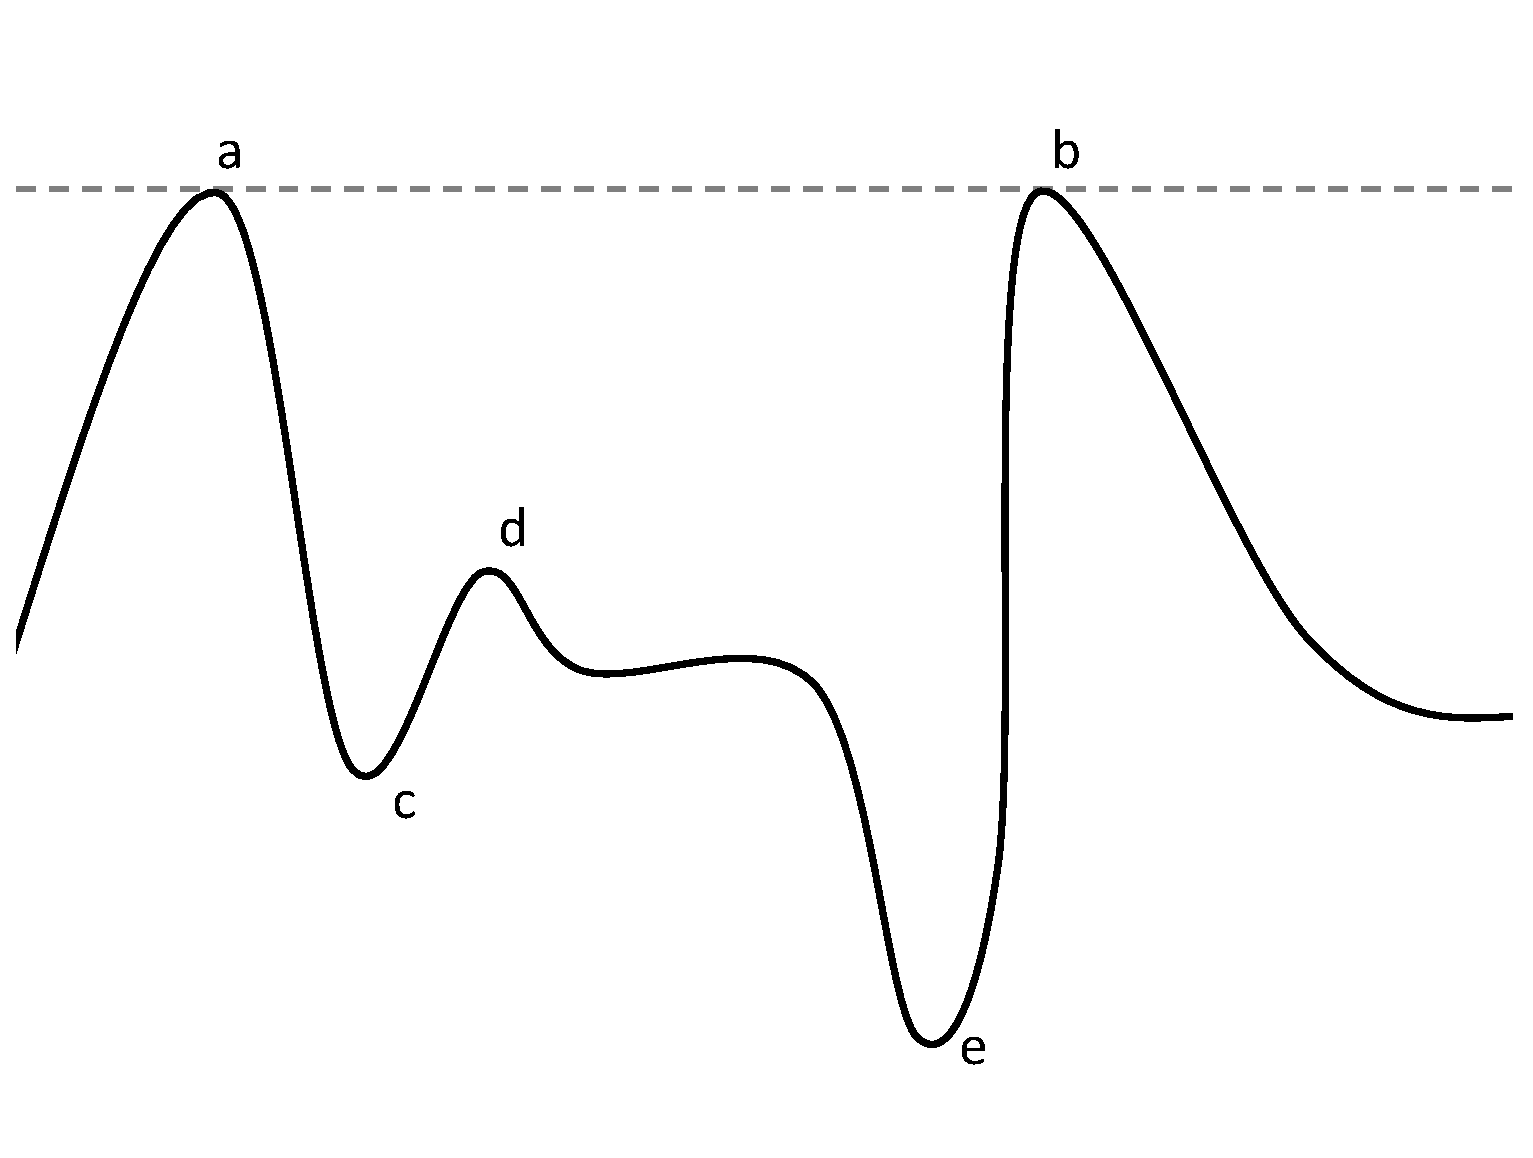
\includegraphics[width=0.4\paperwidth]{searchSpace}
\caption{Examples of local and global optimums.}
\label{localAndGlobalOptims}
\end{figure}

In figure \ref{localAndGlobalOptims}, we can see different examples of global and local optimums. The points labeled \emph{a} and \emph{b} are both global maximums, as they have the same value. The points
\emph{c} and \emph{d} are respectively local minimum and maximum, while \emph{e} is the global minimum.

From all the preceding, we can provide the minimal formulation of an optimization problem as follow 

\definition{Optimization problem}{
\begin{align*}
\text{minimize } &f(x) \\
\text{subject to } &(x \in S)
\end{align*}
Where \emph{S} is the problem search space and \emph{f(x)} the objective function.}

\section{Numerical versus Combinatorial Optimization}

\section{No Free Lunch Theorem}

The No Free Lunch (NFL) Theorems for optimization is a very important result of the field, formalized by Wolpert and Macready \cite{585893}. The basic idea behind these theorems is that no optimization method outperform the others when regarding the class of all the possible problems or, as the authors themselves say,
\begin{quote}
"any two algorithms are equivalent when their performance is averaged across all possible problems." [[give ref on coevolutionnary free lunches]]
\end{quote}
If an algorithm outperforms another on certain types of optimization problems, there must be others classes of problems where this algorithm performs worse.

The NFL theorems are based on several assumptions:
\begin{itemize}

\item the search space is finite

\item the optimization algorithms never re-evaluate the same point

\end{itemize}

The first assumption limit the scope of NFL theorems to the realm of combinatorial optimization, as continuous optimization problems contain by nature an infinity of elements. Indeed, it has been shown that, in the context of continuous optimization, free lunches were indeed possible \cite{Auger-s00453-008-9244-5} (but possibly at the cost of very big memory footprint). Thus this result does not impact directly the scope of this work, but we believe that it is still a good illustration of one of the main problematics of the optimization research field, which is that one must often compromise between [[généralité]] and efficiency. Even in the context of continuous optimization, where the existence of free lunches has been demonstrated, it is probable that we will never find a be-all and end-all optimization technique. This point is for example discussed in \cite{Doe05}.

One example which can be connected to the NFL is the compromise between exploration and exploitation. Basically, an optimization method must often make a compromise between using the previous results to converge toward a region of the search space and exploring the remaining of the search space to find a better region.
For example: some gradient-based methods will use the evaluated points to converge toward a local optimum, but can miss a better solution as they insufficiently explored the search space. On the opposite, some others methods can make a throughout exploration of the search space (by partitioning or random drawing points), but will be slow to converge towards the exact optimum.
It is often possible to parametrize the method to tune the compromise between exploration and exploitation regarding the nature of the problem at hand but, once more, a relevant parametrization requires a sufficient knowledge of the properties of the problem.

Of course, the NFL theorems consider \emph{all the possible objective-functions}. One could argue that "interesting" problems (at least from en engineering point of view) are not distributed evenly over such a space, but correspond to a subset for which some optimization methods are more efficient than others. This is why optimization as a scientific research domain make sense. 

This distinction has been formalized by differentiating \emph{incompressible} from \emph{compressible} objective-functions. Incompressible objective-functions are random and it is thus impossible to develop an optimization method to find the solution efficiently, since good and bad values are randomly distributed. Of course, such "impossible" objectives function make for the major part of all the possible objective-functions \cite{English:3-540-45356-3_7}.
As we said, the set of "interesting" objective-functions, or even the set of real-world related ones is much much more restrained. And for this specific category, some optimizers are better than others. 
However, as we will see in the next sections, the variety of "interesting" optimization problems is still important enough to have resulted in a great variety of specific optimization techniques.

One consequence of the NFL is that selecting an efficient optimization method for a given problem requires to have at least a minimum insight on the properties of the problem. No algorithm can be deemed most efficient for the general case.

On a side note, it can be added that, in addition of the case of continuous optimization, the possible existence of free lunches has been demonstrated for coevolutionary \cite{1545946} as well as multiobjective optimization \cite{1299403}.

\chapter{Numerical Optimization}

As we have seen at the end of the last chapter, optimization methods have to make various compromises regarding applicability versus efficiency.  A great variety of methods exits in the literature, from generic methods applicable to a great variety of optimization problems to very specialized methods designed to be efficient in a specific context. These methods can be segregated by the type of problems they aim to solve or some inherent properties of the method.

Some possible criteria to discriminate based on the type of problem:
\begin{itemize}
\item can we obtain derivatives of the functions defined?
\item is the problem linear (or possibly quadratic)?
\item is the problem convex?
\end{itemize}

For the method in itself:
\begin{itemize}
\item is the method able to take in account constraints on the problem?
\item does the method provides a global solution or a local one?
\item is the method deterministic or stochastic?
\end{itemize}

Based on the shape of the search space and our requirements regarding the method, we will try to choose the most adequate optimization method. As always, the more information known regarding the problem, the more we would be able to select a specialized method with a great efficiency. If very few information is known, it could be necessary to use black-box optimization methods, that is methods which do not make assumption regarding the nature of the problem. These techniques can suffice in themselves to get a good-enough result, or can be used as a prelude of more specialized techniques if enough information is gathered.

A rough proposal of organization of the different types of numerical optimization can bee seen in \ref{numerical_optim_tree}.

\begin{figure}
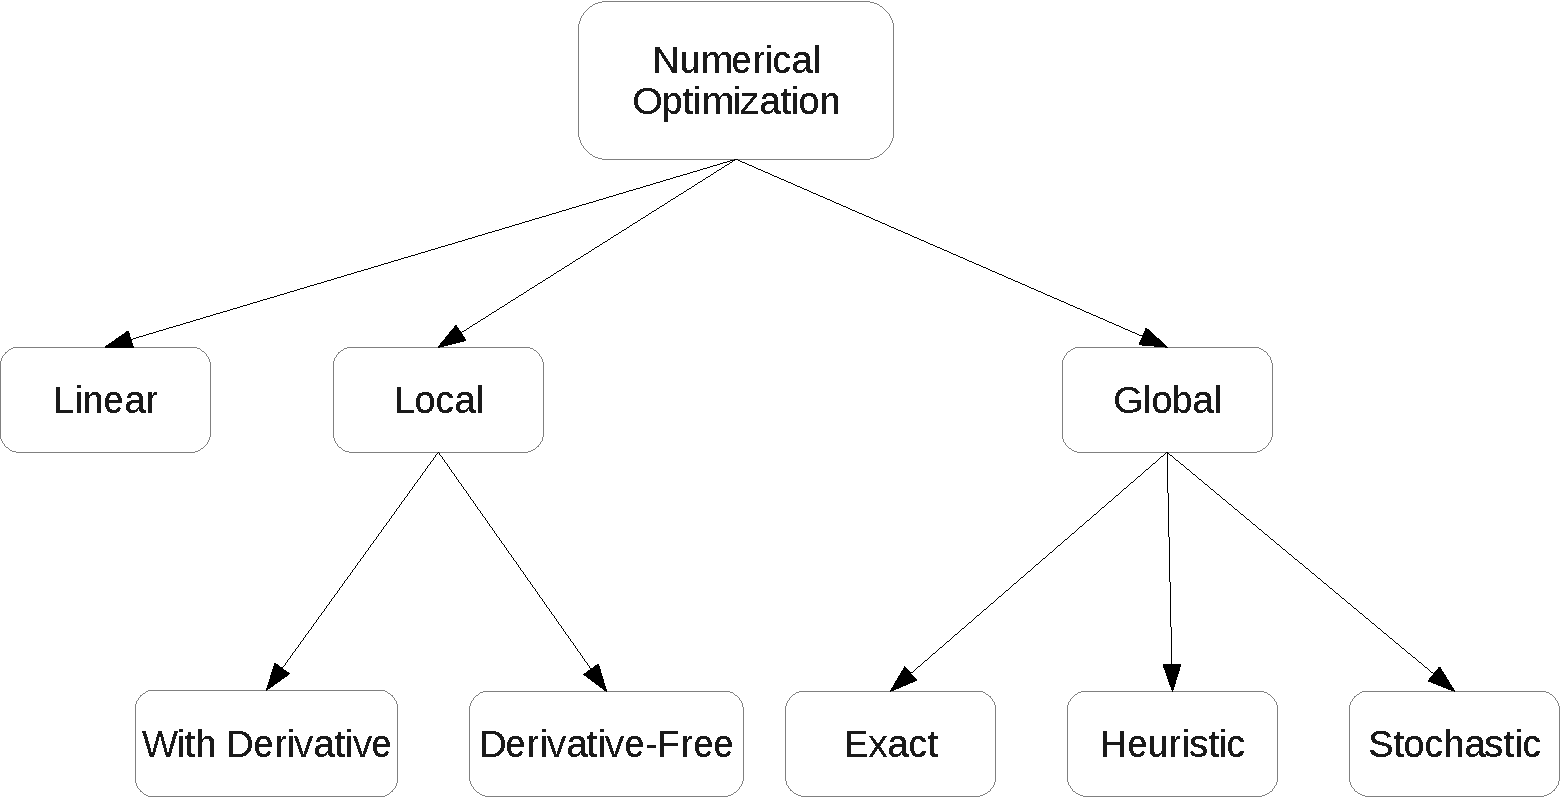
\includegraphics[width=\textwidth]{numerical_optim-crop}
\caption{Types of numerical optimization methods}
\label{numerical_optim_tree}
\end{figure}

Presenting all the numerical optimization techniques would be far outside the scope of this work. In this part we will focus on presenting briefly the different optimization categories we identified on figure \ref{numerical_optim_tree}. We will reference some of the most representatives techniques to illustrate his presentation, but without going into the details of the the techniques. To get a more throughout view of the different techniques, the reader can see reference works such as [[REFS]].

\section{Linear Optimization}\label{linear_optim}

Linear optimization focus on the solving of problems where the objective-function and constraints are linear (that is, $f(x+y) = f(x)+f(y)$ and $f(ax) = af(x)$) and the search space convex.

[[Show what do we mean by convex search space]]

A linear problem with $n$ variables and $m$ constraints can be expressed as:
\begin{align*}
\text{min } & c_1x_1 + c_2x_2... + c_nx_n\\
\text{subject to } &x_i \geq 0, \forall i \in 0,n\\
&a_{11}x_1 + a_{12}x_2 + ... + a_{1n}x_n + b_1 \geq 0\\
&...\\
&a_{m1}x_1 + a_{m2}x_2 + ... + a_{mn}x_n + b_m \geq 0
\end{align*}

This kind of problems is the most basic one. The most well-known method to solve linear problems is the Simplex algorithm\cite{dantzig2003linear}, published by Dantzig in 1947 (based on the work of Leonid Kantorovich). The Simplex algorithm is considered to be the first formal algorithm to solve a numerical optimization problem and to be one of the founding works to the field.

The basic idea of the simplex algorithm is to that the solution space is the convex polyhedron, and the optimal solution is necessarily on one of its vertices. Another property is that a vertex which is not the optimal solution will have at least an edge leading toward a better vertex.
The simplex algorithm starts on one of the vertices, and tries to follow an edge to a vertex which improves the objective-function. The algorithm iterates until it has found a vertex with no edge leading toward a better point (the optimal solution) or until it reaches an unbound edge (in this case the problem is not bounded).

While the simplex algorithm is considered to be very efficient for most cases, some alternatives has been proposed. The most noteworthy is the interior point method and its derivative. Contrary to the simplex method, this methods actually traverses the interior of the solution space (hence its name). The original method proposed by Karmarkar\cite{Karmarkar:1984:NPA:800057.808695} travels through the search space by iteratively finding the best solution over a restricted region delimited by a sphere around the current point.

\section{Local Methods}

Unconstrained local optimization methods concentrate on finding local optimums either because the search space is too big or to complex to find a global optimum in a reasonable time, or because we prefer to quickly find a good enough solution to spend more time to find the best one.
 Moreover, if the objective-function is convex, the local optimum is also the global optimum, in this context local methods can be an easy mean to obtain the best solution.

\subsection{Using Derivatives}

If the derivatives are available, it is possible to propose very efficient optimization techniques to converge toward a local optimum.

In some case, even if the derivatives are not available, it is possible to obtain an approximation of the derivatives using for example a finite difference method. The basic idea of finite difference is to estimate the derivative from the ratio between the variation of the input and the variation of the output of the function.
Basically, if we make the following assumption:

\begin{equation*}f(x + d) \approx f(x) +df'(x)\end{equation*}

then we can estimate the derivative as follow:

\begin{equation*}f'(x) \approx \frac{f(x + d)  - f(x)}{d}\end{equation*}

\subsubsection{Without Constraint}

Methods of this kind can be mostly classified in to broad families: line search and Trust region.
Both families are iterative approaches but differ in the information they use to select the next search point.

The general idea is, from a random starting point $x_0$, to iteratively evaluate a new point using a direction and a step size.
By adjusting the ways the direction and step size are chosen, we can obtain a whole selection of algorithms with varied behaviors.

Formally, from the point $x_i$, the new point $x_{i+1}$ is calculated with:

\[ x_{i+1} = x_i +s_id_i \]

where $d_i$ is the direction vector and $s_i$ the step size coefficient.

\paragraph{Line search}

Linear search is the most basic approach. It first determine  which direction would improve the objective function, then decide of a step size to move toward it.
Some of the most well-known linear search methods are gradient descent, Newton's and Quasi-Newton methods. The gradient method simply uses a step size proportional to the value of the gradient. The Newton's and Quasi-Newton methods however try to find a solution to the equation $\nabla f(x)=0$. The Newton's method use the gradient  and the Hessian matrix of $f$ to estimate a good step size, while the Quasi-Newton method avoid the disadvantages of using the Hessian (which can involve costly operations) by replacing it with an approximation based on the variation of the gradient.

\paragraph{Trust region}

Trust region methods use the neighborhood of the current point to approximate the shape of the objective-function in the neighborhood of the current point. This approximation is the used to find the minimum in a localized region around the current point. These methods are the dual of Line search ones as they start by selecting a step size (the size of the region around the current point) and only after choose the direction.
For example, the Levenberg-Marquardt algorithm, which primary application is least squares problems, uses the Jacobian matrix conjugated with a damping factor to iteratively refine the approximate functions.

\subsubsection{With Constraints}

One of the first proposal for solving constrained problems with derivative is a generalization of interiors points (presented in \ref{linear_optim}). The idea is that a linear function with a non-convex search space can be transformed into a linear function over a convex search space (which is a requirement for applying interiors points techniques), using \emph{self-concordant barrier functions}.
[[BARRIER FUNCTION - WE WILL TALK ABOUT THIS LATER -> MENTION IT ?]]
[[PICTURE OF BARRIER FUNCTION ??]]

A barrier function is a function whose value increases to infinity when its input approaches a fixed boundary.
The idea is to replace the constraint with a barrier function, which is composed to the objective-function. The barrier function is thus used as a penalty for a point which violate the constraint.

For example, taking the following constrained optimization problem:

\begin{align*}
\text{minimize } &f(x)\\
\text{ subject to } &x > 0
\end{align*}

Suppose we are provided a barrier function $b_c(x)$ those value increase toward infinity as x decreases toward 0 ($\lim_{x \to 0^+}b_c(x) = \infty$). We can now use the new unconstrained optimization problem:

$$\text{minimize } (f_{obj}(x) + b_c(x))$$

Another method, which had for some time dominated this part of the numerical optimization field is Sequential Quadratic Programming (SQP). SQP proposes to replace the problem to solve by a sequence of quadratic problems, usually more easily solvable.
SQP is based on a very powerful result of numerical optimization, the Karush-Kuhn-Tucker (KKT) conditions. The KKT conditions are necessary conditions for a solution $x*$ in a nonlinear optimization problem to be a local optimum. They state that, for $x*$ to be a local optimum to an optimization problem with $i$ inequality constraints $gi$ and $j$ equality constraints $h_j$, there must exist some $\mu_i$ and $\lambda_j$ such as:

$\left\{
 		 \begin{array}{l}
			\nabla f(x*) + \sum \mu_i \nabla g_i(x*) + \sum \lambda_j \nabla h_j(x*) = 0 \\
			g_i(x*) \leq 0 \;\forall i \\
			h_j(x*) = 0 \;\forall j \\
			\mu_i \geq 0 \;\forall i\\
			\mu_ig_i(x*) = 0 \;\forall i
		\end{array}
	\right. $
	
The SQP can be viewed as an equivalent of Newton's method to the KKT conditions of the problem.



\subsection{Derivative-Free}

Sometimes we cannot use derivatives in the optimization process, either because the derivatives are not available or too costly to compute.

A very popular method is the Nelder-Mead algorithm. This algorithm places a simplex\footnote{The concept of simplex is a generalization of the concept of triangle in arbitrary dimension. A triangle is a simplex in 2 dimensions, a tetrahedron a simplex in 3 dimensions.It should be noted that the Simplex algorithm, presented in \ref{linear_optim} does not actually use simplices, during solving.} on the search space and applies to it a sequence of transformations by moving its edges.

[[TODO: Picture of Nelder Mead ]]

At each iteration, a new test point is calculated (for example the symmetric of the worst vertex of the simplex regarding the gravity center of the others points). If this point is better than every vertices, then the simplex is stretched toward it. If this point is worse than the current vertices, then we suppose we are stepping over the valley which contain an optimum. In this case the simplex is contracted to be able to explore the valley. Else, we simply replace the worst vertex by the new point.
The iterations stop when the simplex has reach a specified size.


Several derivative-free algorithms interpolate the objective-function with a simpler one. Starting with several evaluation points of the objective-function, we build a simpler function to which we can apply a known optimization method. Based on the result of the optimization, we can update the interpolation model and reiterate.
[[Talk about possible interpolations methods ?]]

\section{Global Method}

While local optimization methods aim only at finding an optimum into a limited part of the search space, global optimization methods aim to find the globally best solution of the problem. Global optimization methods concentrate on providing strategies to explore the search space.

Depending on the nature of the problem, it may be impossible to guarantee that the best solution will be found by any mean other than a complete exploration of the search space (which is in itself an impossible task in the context of continuous optimization).

For example, suppose the following problem:

Minimize $f(x) =$ \begin{cases}
 		 					0& \text{if } x = 1 \times 10^{-9}\\
 		 					1& \text{otherwise} 
 		 			\end{cases}
 		 			
There is no efficient strategy to find the global optimum to such a problem (unless knowing the equations, a thus the solution, beforehand).

Consequently, obtaining the global optimum of an optimization problem with certainty will be possible or not depending on the properties of the problem.
As with local optimization methods, several kinds of approaches have been proposed to solve problems with different properties.

\subsection{Exact Methods}

These methods aims to provide a guarantee about the optimality of the solution. These methods cannot used for any optimization problem, as they need to use some properties of the problem to prove that the solution is a global optimum.

For example, as we said before, if an optimization problem is convex than a local solution is also a global solution. Consequently for convex problem local optimization methods can be used with the guarantee that the solution found will be the best one.

[[
Branch and Bound

Taboo search
]]

\subsection{Stochastic Methods}

[[
Simulated Annealing

Monte-Carlo
]]

\section{Conclusion on Numerical Optimization}

This overview of numerical optimization illustrate how the different optimization techniques range from very efficient but highly specialized methods to board scope methods with slower and more costly strategies.

[[Two axis: Local <-> Global; Specialized <-> Generic]]

\chapter{Multi-Objective Optimization}

Multi-objective optimization (MOO) departs significantly from previous categories of optimization in the fact that you have to consider multiple objective functions instead of one. A main aspect of MOO is the way to conciliate these objectives, which are usually contradictory.
An example of real-world everyday MOO problem could be choosing the mean of transportation for a travel, trying to find a balance between speed and cost. Airplane is the fastest way of transportation, but is expensive. While car is slower, it is cheaper. Train is slower than plane, more expensive than car, but can preferred as the best compromise. There still, however, are solutions which are strictly worse than others (in our example, renting an helicopter would probably be both more expensive and slower than buying a seat on a commercial airplane).
From this example we can see that, for a MOO problem, there rarely is a clear-cut "best" solution. And more importantly that even some solutions which are not optimum for \emph{any} of the objectives can be deemed satisfying. Only when each objective is completely independent, or when no objective is contradictory to another, then a MOO problem can be handled as a set of separated mono-objective optimization problems.
A solution vector which would be optimum for each objective is sometimes called \emph{utopia point}, or \emph{shadow minimum}, and is used as a reference comparison in some of the MOO techniques we present.

[[FORMULATION OF A MOO PROBLEM]]

MOO problems are quite a radical departure from previous optimization problems type we have seen. Many approaches have been proposed, the majority of which can be separated in to categories: \emph{a priori} and \emph{a posteriori} approaches. A priori approaches aims to discriminate between the objectives \emph{before} the optimization process. This often consist into combining the different objectives into one, before applying a classical optimization method on the new, aggregated objective.
On the opposite, a posteriori methods tries to provide a set of efficient solutions among which the decider will choose.
A priori approaches are considered easier, but not very efficient, whereas a posteriori approaches provides more diversity of solutions as well as more insight about the nature of the problem.
A third category can also be considered: the \emph{interactive} methods. Basically, these methods iterates between decision and search phases. For example, an interactive  method could work by quickly providing intermediate solutions to the decision-maker, which would in return refine the search using them.

We will now see some of the strategies have been proposed to deal with such a type of problem.

\section{A Priori Methods}

\subsection{Objectives Aggregation}

The first approach is to transform the MOO problem back to a mono-objective optimization problem, by aggregating the different objectives into one. This can be expressed as follow : \(f_g = aggr(f_1, f_2, ..., f_n)\), where \(f_1, f_2, ..., f_n\) are the original objectives and \(f_g\) the aggregated one, which will be used with classical mono-objective optimization methods.

Concerning the choice of the aggregation function, different strategies can be used.

Concerning the choice of the aggregation function, the simplest strategy is to use a classical function such as addition, multiplication, mean, max or min of the objectives, and variations of the preceding (exponential sum, ...): these methods present the major drawback of requiring the aggregated values to be comparable.[[ Keeping with our travel example]], is it relevant to simply add duration and cost ?

A slightly more sophisticated way is to use pondered mean: we attribute a coefficient to each objective when adding them :

\[ f(x) =\sum_{i=1}^n w_i f_i(x) \]

Where $w_i$ are the coefficients representing the relative preferences between the objectives.

This method allows to express a preference between different objectives, as well as bringing back on comparable scale different objectives. However, one now has to decide of the coefficients to choose. Also, this method can hide some information concerning the solution, for example an extremely poor result in one of the objectives, compensated by small improvements in all the others.  [[Moreover, this solution present some limitations when the solution space is nonconvex [[EXPAND]]]]

[[To get refs which criticize Weighted sum, see "Survey of multi-objective optimization methods for engineering"]]

\subsection{Lexicographic Method}

In this method, the objectives functions are arranged and optimized by order of importance. The result of the optimization at a given step become a constraint to satisfy for the following steps.

Formally, the problem become an ordered set of optimization problems expressed as follow:

\begin{align*}
\text{min } &f_i(x) \\
\text{subject to } &f_j(x) \leq f_j(x_j^*) \\
j = &1, ..., i-1
\end{align*}

A variation of this method proposes to replace inequalities by equality constraints. [[REF]]

Another variation, sometimes called hierarchical, introduces a constraint relaxation coefficient $\delta$ where the new formulation of the constraints becomes:

\[ f_j(x) \leq \left(1 + \frac{\delta_j}{100}\right) f_j(x_j^*) \]

\subsection{$\epsilon$-constraint Method}

The $\epsilon$-constraint method proposes to change the expression of the problem by keeping only one objective (the one deemed the most important) and transforming the others into inequality constraints.

For example, the problem \[\text{min } f_1, f_2, ...,f_n\] where $f_1$ is deemed the most important objective would be transformed in
\begin{align*}
\text{min } &f_1 \\
\text{subject to } &f_2 \leq \epsilon_2, ..., f_n \leq \epsilon_n
\end{align*}

Where $\epsilon_2, ..., \epsilon_n$ must be chosen by the designer.
Depending of the selection of $\epsilon_2, ..., \epsilon_n$, it is possible to obtain a formulation where no feasible solution exist.
[["Survey of multi-objective optimization methods for engineering" -> Bounded objective function method for some ref about methods to select $\epsilon$]]

\subsection{Goal Programming}

[[REF in "Survey of multi-objective optimization methods for engineering"]]

The idea of Goal Programming (also called Target Vector Optimization) is to fix for each objective an associated goal to reach. Each objective can be over- or underachieving its goal, allowing the designer to provide a rough idea of the initial design goals.

The new objective is to minimize the total deviation $\sum_{i=1}^n |f_i - g_i|$ where $g_i$ is the goal associated to objective $f_i$.

Goal Programming is very easy to use and quite popular, and can work even when the designer provided some unreachable goals, but provides no guarantee for the optimality of the solution.

\subsection{Min-Max Method}

This method use the separately attainable minima of the objectives (the so-called \emph{utopia point}) and try to minimize the maximum deviation of the objectives relative to those minima:

\[ \text{min } f = \text{ max } \left( \frac{f_i - f_i^0}{f_i^0} \right) \]

where $f_i^0$ represent the separately attainable minimum of the objective $f_i$.

This method can also be used similarly to Goal Programming, where the separately attainable minima are replaced by goal given by the designer.

A variant of this method, called weighted min-max, or Tchebycheff method, use the following formulation:

\[ \text{min } f = \text{ max } w_i |f_i - f_i^0| \]

where $w_i$ are coefficient provided by the designer.

[[Talk of variants ??]]

\subsection{Analysis of a priori methods}

A priori methods provide a simple and efficient way to tackle the problem of multiple objectives, as they allow to reduce the problem to a mono-objective one.
However, a drawback of these methods is the need for the designer to have a good knowledge of the problem, to know the correct way to combine/compare the different objectives functions. In the general case, the designer could not have enough experience or information to make such decision.

In the case where the designer would have enough knowledge to meaningfully use such a method, the introduction of this knowledge can risk to introduce a bias in the resulting solution, orienting the optimization process toward "standard" solutions at the expense of possible non-conventional ones.

Moreover, aggregations techniques tend to break when the objectives are not comparable, requiring once more knowledge from the designer to introduce adjustment coefficients to re-equilibrate the aggregation function.

\section{A Posteriori Methods}

We have seen that, while convenient, \emph{a priori} methods can be quite restrictive. By choosing beforehand a way to aggregate the objectives, we lose in diversity of solutions and influence the result of the optimization process.

\subsection{Pareto Dominance}

A radically different approach has be proposed, using the concepts of Pareto dominance and Pareto optimality. These concepts were originally been developed in economical sciences first by Francis Edgeworth and later Vilfredo Pareto. The initial application of the concepts was to propose a minimal definition of "efficiency", regarding allocation of resources inside an economical system.

The main idea is that a state where it is impossible to improve the resources allocation for an individual without worsening the situation of at least another is described as \emph{Pareto efficient}, or \emph{Pareto optimal}.

Conversely, if from a system state A it is possible to find a new state B where at least one individual's situation is improved without worsening the situation of another, the state A will be said to be \emph{Pareto inefficient}. The state B will be said to \emph{dominate} the state A in terms of Pareto optimality, and the passage from A to B will said to be a \emph{Pareto improvement}. This relation of Pareto dominance is usually noted \(\prec\).

\definition{Pareto-dominance}{Given A and B two vectors describing different resources allocations in a system, \(A \prec B \Leftrightarrow (\forall i \text{ }A_i \leq B_i \land \exists j \text{ } A_j < B_j\)). }

Note that in the preceding example, we wanted to maximize resources allocation, so \(A \prec B\) reads " B dominates A". If we want to \emph{minimize} the allocation, the meaning is inverted and  \(A \prec B\) reads "A dominates B".
As it is the standard convention in optimization to express problems in terms of minimization, for the rest of this thesis we will use \(A \prec B\) with the meaning of "A dominates B", unless otherwise specified.

Based on this relation of dominance, it is possible to provide a definition of Pareto-optimality.

\definition{Pareto-optimality}{A solution vector that is dominated no other possible solution is said to be Pareto-optimal.}

\definition{Pareto front}{the set of Pareto-optimal solutions.}

It is also possible to classify the solutions by rank: a solution which is dominated by no other is said to be of rank 0 (and to be Pareto-optimal). A solution which is dominated by at most a solution of rank 0 said to be of rank 1 and so on.

As a remark, these definitions of efficiency and optimality do not give any information about the fairness of the allocation, or the well-being of the involved parties. From this point of view, a monopolistic situation where one actor would control all the available resources is as optimal as a situation where all the resources are equally divided between the individuals.

These definitions of dominance and optimality can be used to characterize the possibles solutions of MOO problem. In this case, the problem is no more to find an optimal solution, but to find the Pareto front of the problem.

An illustration of Pareto front can be seen on figure \ref{Front_Pareto}. The elements A and B are Pareto-optimal, while C is not.


\begin{figure}
\centering
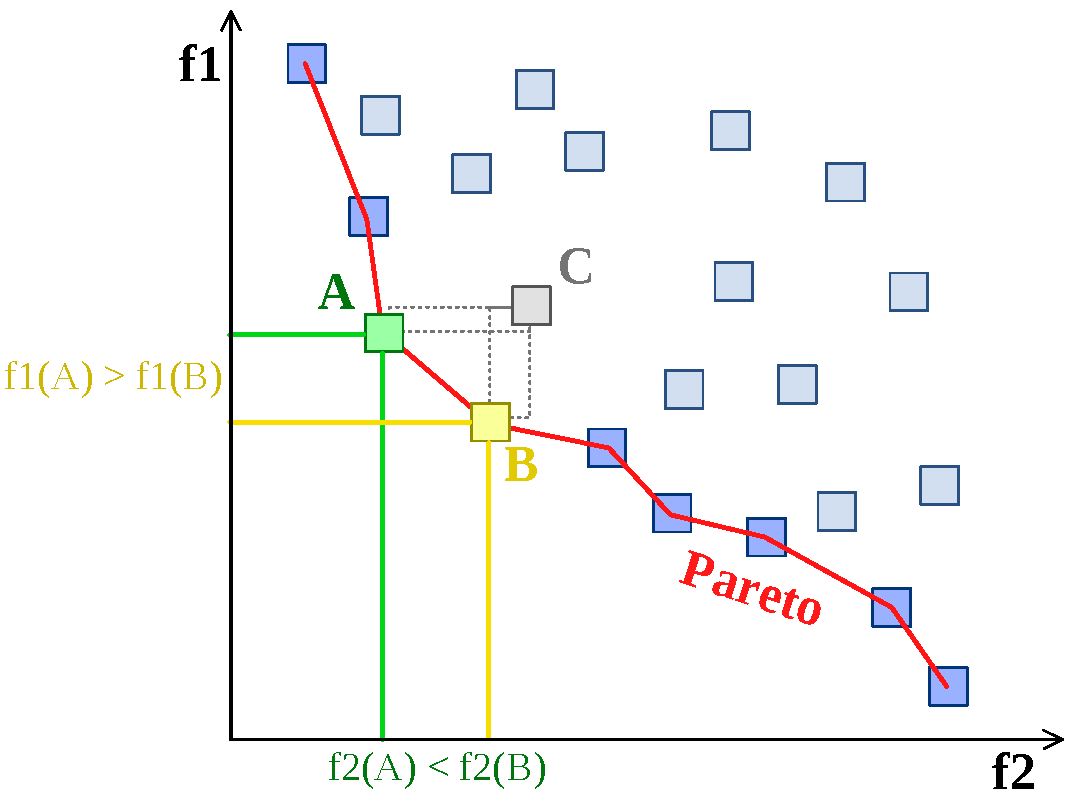
\includegraphics[width=0.4\paperwidth]{Front_pareto}\\
%\hfill\includegraphics[width=6em]{by-sa} \href{http://en.wikipedia.org/wiki/File:Front_pareto.svg}{\begin{small}Johann Dréo\end{small}}
\caption{Illustration of the notion of Pareto Front (CC-BY-SA \href{http://en.wikipedia.org/wiki/File:Front_pareto.svg}{Johann Dréo)}}

\label{Front_Pareto}
\end{figure}

[[TODO: give some example of Pareto methods]]

\subsection{Transforming A Priory Approaches}

A first possibility is to use an a priory method and iterating over it while varying the different parameter to obtain a set of solutions.

[[Example Weighted sum]]

\subsection{Normal Boundary Intersection Method}

Normal Boundary Intersection (NBI)\cite{S1052623496307510} method provides a even distribution of Pareto-optimal solutions using a parameter vector $w$ provided by the designer.

The method use 

[[Explain it]]

One drawback of NBI is that it can produce solutions sets which contain non Pareto optimal-points, as well as overlook some points which are Pareto-optimal.

\subsection{Normal Constraint Method}

Normal Constraint (NC) method tries to improve on NBI by introducing a Pareto filter to avoid the selection of non Pareto-optimal points.

\subsection{Evolutionary Algorithms}

[[Talk about scalability problems -> "Techniques for Highly Multiobjective Optimisation: Some Nondominated Points are Better than Others" by David Corne and Joshua Knowles]]


A widespread strategy to find the Pareto front is to use [[population-based]] metaheuristics, such as Multi-Objective Evolutionary Algorithms (MOEA). 

Historically, evolutionary algorithms are divided in two main categories, based on whether or not they use elitism mechanisms, with some consensus concerning the superiority of elitist algorithms.

\subsubsection{Non-elitist evolutionary algorithms}

[[Vector Evaluated Genetic Algorithm (VEGA) Schaffer (1985) => Non Pareto]

[[  Goldberg and Richardson (1987) =>  Simple Pareto domination scheme. • Sharing on whole population]]


\subsubsection{Elitist evolutionary algorithms}

Different possibilities has been explored to introduce elitism in MOAE. A common approach is to use a second population consisting of elite, non-dominated individuals, which are used as recombination partners for the main population.

[[Signal that evolutionary algorithms have difficulties with more than two objectives ?]]

\section{Interactive Methods [[?]]}

\chapter{Optimization under Uncertainties}

In a pure mathematical world, all models are perfectly correct and have an infinite precision. However, in the physical world, our knowledge can be extremely limited. Moreover, high precision models can require a long time to be computed, making them prohibitively costly when used in the context of an optimization process. At last, when the optimization problem is complex, a small approximation can result in large variations of the output, if the system is sensitive to parameters variations.

[[ILLUSTRATE THE SENSIVITY PROBLEM WITH AN EXAMPLE]]

In order to tackle these issues, several works have been done to take in account uncertainties into the optimization process. We propose to make a quick tour of the different ways which have been propose to model and propagate uncertainties.
A major concern regarding the modeling of uncertainties is the uncertainties \emph{propagation}. 

\section{Several types of uncertainties}

[[TALK ABOUT system vs experimental vs modeling uncertainties ?]]

A distinction is usually made between \emph{aleatory} uncertainties and \emph{epistemic} uncertainties.

Aleatory uncertainties are inherent to the studied system. They can represent for example variability in the material used, a physical variation regarding the manufacturing of some piece, the meteorological conditions to which a device will be exposed etc.
These uncertainties are \emph{irreducible} as it is impossible to remove them with a better analysis of the system.

Epistemic uncertainties result from an incomplete knowledge regarding the system. These uncertainties can result from a limited set of data or lack of knowledge regarding a physical phenomenon.
The uncertainties are \emph{reducible} as it is possible to remove them with a better analysis of the system. However, removing epistemic uncertainty can often be too costly or too difficult in practice, thus still need to be taken in account during the optimization process.

For example, let's suppose we work on a model taking two variables as input and producing an output: $z=f(x,y)$.
Based on known uncertainties on the inputs and the model, how easy it is to combine and propagate these information to determine the uncertainty regarding the output ? Or more formally, can we provide a propagator $P$ such as $u_z = P(u_x, u_y, u_f)$ (where $u_i$ is the uncertainty associated with the element $i$)? As we will see, the ease to obtain such a propagator $P$ depends on the chosen way to model the uncertainties.

\section{Uncertainties Modeling Techniques}

\subsection{Probability Theory}

[[Dans la mise en oeuvre, dire qu'on a utilisé celle là comme exemple parce que c'est la plus commune, qu'elle est bien comprise, et qu'il est facile de trouver des outils pour la manipuler]]

Using the probability theory, uncertainty can be modeled using a distribution function. This modeling provides the advantages of a well-studied theoretical foundation, providing well-known combination and propagation techniques.

Aleatory uncertainties can be characterized by obtaining a distribution function from a data sample.
Well-known statistical techniques can be used to see for example if a data sample follows a known probability distribution, measuring \emph{goodness of fit}, that is, how well a data sample follows a given model, such as the Kolmogorov-Smirnov test \cite{Massey_1951}. 
However, care must be taken as these techniques can introduce some more epistemic uncertainties which can lead to misleading results (for example in the case of insufficient data samples).

Concerning epistemic uncertainty, it can be more difficult to estimate a relevant distribution function  [[TO EXPAND]]

\subsection{Interval Analysis}

Interval analysis can be an alternative to probability theory when the lack of information impeded modeling with a probability distribution, but where the uncertainty can still be bounded within a certain domain.
How easy it is to propagate intervals depends on the involved models. For example in the case of a monotonic function the lower and upper bounds can be determined easily. In the general case, determining the boundaries is equivalent to solving an optimization problem and can thus be solved by using optimization algorithms. In the most extreme cases, one can apply sampling techniques, but this can become quite expensive.
For some examples of existing techniques, one can refer to \cite{Kreinovich_2008}.

A limit of interval analysis is the lack of a measure equivalent to probability, which limit the [[interest]] of this representation in the general case. This modeling can still prove useful in the context of worst case studies where inputs variables can be bounded with accuracy.

\subsection{Fuzzy Sets}

[[Add some ref]]

Fuzzy Sets can be seen as a compromise for when we still lack enough information to use probability theory, but we have more knowledge than just the bounds of the uncertainty.

Basically, fuzzy sets are sets where the membership of an element to the set is not absolute but gradual.
In classical set theory, an element is or is not a member of a set. This notion can be formalized as a function $f_S: X \rightarrow \{0,1\}$ where 
$\left\{
 		 \begin{array}{rcr}
			f_S(x) = 0 \Leftrightarrow x \not\in S\\
			f_S(x) = 1 \Leftrightarrow x \in S
		\end{array}
	\right. $

In the context of fuzzy sets, the equivalent function could be formalized as $f_S: X \rightarrow [0, 1]$, where $f_S(x)$ represents the degree of membership of $x$ to $S$. A value of 1 indicates a total membership to S, a value of 0 a complete absence of membership to S and the values in between specific degrees of membership.
In this regard, fuzzy sets can be seen as a generalization of classical sets.

Fuzzy Sets quantification capability to represent vague information make it attractive to model epistemic uncertainty, as it is more precise than interval analysis and well-suited to express expert knowledge. However this modeling is less powerful and expressive than probability theory, lacking for example a mean to represent an uncertainty measure equivalent to the probability of the probability theory. Indeed, the membership function is insufficient to characterize the likelihood of non-connected events.
To overcome this limitation, the fuzzy set theory was extended into the possibility theory.

\subsection{Possibility Theory}

[[Add some ref]]

Possibility theory seems similar to probability theory. However, they are based on axioms which diverge on a fundamental point.
The probability theory is based on the axiom of \emph{additivity}, which says that for two disjoints sets $U$ and $V$, $P(U \cup V) = P(U)+ P(V)$, that is the probability of at least one of two mutually exclusive events to be verified is the sum of the probabilities of each event.

The possibility theory contains instead an axiom of \emph{sub-additivity} saying that for two disjoints sets $U$ and $V$, $\Pi(U \cup V) = \text{max }(\Pi(U), \Pi(V))$ (where $\Pi(X)$ reads as "possibility of X").

Let's take the basic example of a door which can be either open or closed. If we assume "the door is closed" has a probability of 1, it must follow that "the door is open" has a probability of 0, since the sum of these two complementary events must be 1.

In the context of possibility theory, if we state that the possibility of "the door is closed" is 1, it is not incompatible with the possibility of the door to be open to be, for example, 0.4.

The intuition behind this difference is that probability theory applies to the reality, while possibility theory applies to the knowledge one has regarding the reality, taking in account the "fuzziness" of one's knowledge. To cite the definition proposed by Nikolaidis et al. \cite{nikolaidis:386}:
\begin{quote}
"Possibility measures the degree to which: a) A person considers that an event can
occur, or b) The degree to which the available evidence does not contradict the
hypothesis that the event can occur."
\end{quote}

As well as the notion of \emph{possibility}, possibility theory introduces the notion of \emph{necessity}. Basically, $Nec(U) = 1 - \Pi(\bar{U})$.
This definition implies several interesting properties:

$\left\{
\begin{array}{l}
Nec(U) \leq \Pi(U)\\
Nec(U) + \Pi(\bar{U}) = 1\\
\text{either } \Pi(U) = 1 \text{ or } Nec(U) = 0\\
\end{array}
\right.$

Necessity and possibility of an event $e$ can be viewed a lower and upper bounds to the probability of $e$.

Possibility theory offers numerous tools similar to the ones of probability theory (so much that it was debated if the two theories are really different or if possibility theory was just a variation on probability theory). However, the capability of this theory to model expert knowledge specifically has made it quite popular in the context of uncertainty modeling.

\subsection{Evidence Theory}

[[Add some ref]]

Evidence theory, also known as Dempster-Shafer theory (DST), takes in account available evidences to provide a degree of belief concerning a fact.
The basic idea of this theory is to represent the notion that, the more evidences seems to confirm a proposition, the more we can belive the proposition is true.

Evidence theory represents a proposition as a set of elements. Thus some propositions can includes others propositions (following the basic set inclusion definition). To these sets are assigned a basic belief assignment (BBA), also called \emph{mass}.

From this mass can be calculated two measures:

\begin{itemize}
\item \emph{Belief:} $bel(S) = \sum_{S'\subseteq{S}} mass(S')$
\item \emph{Plausibility:} $pl(S) = \sum_{S'|S' \cap S \neq \emptyset} mass(S')$
\end{itemize}

The mass measurement represents the amount of evidences which support the proposition, the likelihood of $S$. The belief and plausibility can be seen as lower and upper bounds to this likelihood.

Once again we can obtain some interesting properties regarding these measures:

$\left\{
\begin{array}{l}
bel(S) \leq mass(S) \leq pl(S)\\
pl(S) = 1 - bel(\bar{S})\\
bl(S) + bl(\bar{s}) \leq 1\\
pl(S) + pl(\bar{s}) \geq 1\\
\end{array}
\right.$

As with possibility theory, belief and plausibility can be used as lower and upper bounds for probability.

Several rules have been proposed to combine informations coming from different (potentially conflicting) sources. To see an overview of these proposals, the reader can refer to \cite{sentz2002combination}.

\section{Using Uncertainty for Robust Optimization}

[[GIVE EXAMPLE OF SEQUENTIAL OPTIMIZATION (AS DONE WITH ICA), FOR A SIMPLE OPTIM UNDER UNCERTAINTY TECHNIQUE]]

\subsection{Taguchi Method - The firsts steps of Robust Optimization }

Robust optimization tries to provide a solution which is both good and insensible to small variations of the inputs.

The research on robust optimization has been initiated with Taguchi's robust design methodology[[REF]], aiming at improving the quality of manufactured goods.
In his methodology, Taguchi proposes a three-stages process :
\begin{itemize}
\item System design, where the designers determine the overall structure of the product at a high conceptual level;
\item Parameter design, where the optimal values of the design variables are determined;
\item Tolerance design, which focus on reducing the variability of the  various parameters to fix an acceptable limit to the variability of quality for the product.
\end{itemize}

To help the designers during the parameter design phase, Taguchi introduced several measures, among them the Signal-to-Noise (SN) ratios. These ratios are used to estimate the sensitivity of a performance of the product to variations. Each ratio relate to a possible goal regarding the studied performance: larger the better, smaller the better, on target the best. These ratios are respectively noted $SN_L$, $SN_S$ and $SN_T$.
By simulation or experimentation, one must first produce a data set.

The $SN_L$ and $SN_S$ can be directly calculated as

\[SN_L = -10\text{log}\left( \frac{1}{n} \sum_{i=1}^n \frac{1}{y_i^2} \right)\]
\[SN_S = -10\text{log}\left( \frac{1}{n} \sum_{i=1}^n y_i^2 \right)\]

For $SN_T$, we need first to measure the mean response, given by $\bar{y} = \frac{1}{n}\sum_{i=1}^n y_i$
This mean can then be used to calculate the standard deviation as follows 
\[S = \sqrt{\sum_{i=1}^n \frac{(y_i - \bar{y})^2}{n-1}}\]
[[REALLY GIVE THE FORMULAS OF MEAN AND STD ??]]

 $SN_T$ can then be calculated as
 
 \[ SN_T = 10\text{log}\left(\frac{\bar{y}^2}{S^2}\right) \]
 
To reduce the sensitivity of the solution to noise, the SN ratio must be maximized. To this end, Taguchi use the Design of Experiment, a statistical procedure for determining the effect of multiple inputs on a desired output. [[GIVE A REF ON DOE]]

[[EXPAND ON DOE  ?]]

\subsection{}

\chapter{Optimization in Dynamic Environments}
A special case of optimization is optimization in dynamic environment. In these kind of problems, the objective-function is likely to change with time.
Classical optimization techniques fail to solve this problem as they are not meant to take in account the dynamic of the problem.
These problems require specific optimization techniques able to both find a moving optimum and to follow it when it changes.

\section{Genetic Algorithms}

\chapter{Multidisciplinary Optimization}

Multidisciplinary Design Optimization, often abbreviated Multidisciplinary Optimization (MDO), concerns the optimization of complex systems which involves several interacting disciplines. Each discipline in itself can contain this own variables, objectives and constraints. These problems often involves several of the optimization problematics we examined in the previous [[chapters]] (non-linearity, multiples objectives and constraints, uncertainties etc.) and are usually too complex to be handled by classical optimization methods, as evaluating the global function of the problem would be considered too costly.
These kind of problems are commonplace in the industry, especially in aeronautic and aerospace engineering, where parts of the design are often done by different experts teams. For example [[the designing of]] an aircraft can be formalized as a MDO problem involving several disciplines such as mechanic, aerodynamic, acoustic etc. (see \figurename\ \ref{aero-disc}).

\begin{figure}
\centering
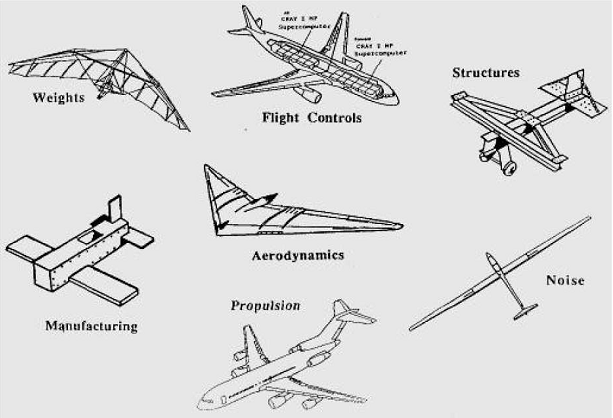
\includegraphics[width=0.4\paperwidth]{Disciplines_Avion}
\caption{Examples of aeronautics disciplines}
\label{aero-disc}
\end{figure}

To handle such complex system, most strategies propose to decompose it into several sub-system of lesser complexity. Concerning engineering, several decomposition strategies have been proposed [[REF Decomposition and Representation Methods in Mechanical Design]]:

\begin{itemize}
\item product (also called object) decomposition, based on the physical components of the system. This kind of decomposition is not always adequate and often subjective;
\item process  (also called sequential) decomposition, based on the work-flow of elements/informations involved into the design process. This decomposition is most adequate when the design process is linear.
\item domain (also called aspect) decomposition, based on the knowledge domains, the disciplines, involved. This kind of decomposition is the basis of MDO methods.
\end{itemize}

[[The AIAA MDO Technical Committee proposed the following definition of MDO\footnote{\url{https://info.aiaa.org/tac/adsg/MDOTC/Web\%20Pages/aboutmdo.aspx}} [[\cite{american1991current}?]]:
 \begin{quote}
"A methodology for the design of complex engineering systems and subsystems that coherently exploits the synergism of mutually interacting phenomena."
\end{quote}]]
MDO methods are not optimization methods \emph{per se}. Instead they focus on providing a optimization strategy for optimizing the different disciplines while maintaining a global coherence. In fact, the optimization of the disciplines is done using classical optimization methods such as presented above. [[In this regard, MDO methods could be seen as optimization meta-methods, or methodologies, as they provide methods to best apply optimization methods to a complex problem. Martin and Lambe\cite{Lambe:2011:A} note the volumes of different terms which have been used in the literature :  "architecture, "method", "methodology", "problem formulation, "strategy", "procedure" or "algorithm". While these authors choose to use the term "architecture", we will stick in this work to the designation of "method", not as a disregard for their arguments but solely for the sake of  consistency.  ]] 

Alexandrov and Lewis illustrated their discussion on Collaborative Optimization\cite{NataliaM.:2000:ACA:886733} with the following theoretical test case:

[[Notion of Standard form]]

\begin{align*}
a_1 &= A_1(s, l_1, a_2) \\
a_2 &= A_2(s, l_2, a_1) \\
\text{minimize } &f(s, a_1, a_2) \\
\text{subject to } &g1(s, l_1, a_1) \geq 0 \\
								&g2(s, l_2, a_2) \geq 0
\end{align*}

[[Add graphical representation]]

It can be noted that this formulation does not differ from the formulation of standard optimization problem. Indeed, as noted by Martin and Lambe\cite{Lambe:2011:A}:
 \begin{quote}
 "If we ignore the discipline boundaries, an MDO problem is nothing more than a standard constrained nonlinear programming problem: we must find the values of the design variables that maximize or minimize a particular objective function, subject to the constraints."
\end{quote}
[[As we will see later, this point is one of the funding principles of the work presented in this thesis.]]

A very common strategy used by most MDO methods is to reformulate the problem to \emph{decouple} variables which are shared among the disciplines. 
For example, the following optimization problem:

\begin{align*}
\text{Minimize } f(f_1(x), f_2(x))
\end{align*}

(where $f_1$ and $f_2$ represent two disciplines depending on $x$)

could become :

\begin{align*}
\text{Minimize } &f(f_1(x_1), f_2(x_2))\\
\text{s.t. } &x_1=x_2
\end{align*}

The shared variable $x$ has been replaced by two independent variables $x_1$ and $x_2$, and a new constraint $x_1=x_2$ has been added to ensure the consistency of the design.


Several specific terms are in use in the domain of MDO:

\begin{itemize}

\item \emph{Design variable}: a variable of the problem which can be chosen by the designer. The goal of the optimization process is to find good values for the design variables of the problem. A design variable is said to be \emph{local} (or \emph{private}) if it is relevant to only one discipline, or \emph{shared} (or \emph{public}) if it is used by several of them.

\item \emph{Discipline analysis/Analyser/Simulator}: 

\item \emph{Multidisciplinary Analysis (MDA)}: [[Say that the models can need to be evaluated potentially SEVERAL TIMES during one MDA, to find consistent set of variables]]

\item \emph{Optimizer/Solver}: A classical optimization technique, such as the ones we have seen in the previous chapters. These optimizers can be applied to the problem as a whole or to specific parts.

\end{itemize}



The classical approach to categorize MDO methods was to separate mono- and multi-level methods.
Mono-level methods use a single optimizer and a non hierarchical structure, while Multi-level methods use a hierarchical structure and possibly several optimizers.

[[introduce others ways to separate

=> GENERAL MDO FRAMEWORK of Balling and Sobieszczanski-Sobieski

=> recent works "Multidisciplynary Design Optimization: A Survey of Architectures" says : 

"We now introduce a new approach to classifying MDO architectures. Some of the previous classifications were based on which constraints could be controlled by the optimizer [77, 121]. Alexandrov and Lewis [121] used the term “closed” to indicate that a set of constraints cannot be satisfied via explicit action of the optimizer, and “open” to indicate that it can.
[...]
Tosserams et al. [84] expanded on this classification
scheme by discussing whether distributed architectures used open or closed local design constraints in the system subproblem. Closure of the constraints is an important consideration when selecting an architecture, because most robust optimization software will permit the exploration of infeasible regions of the design space. Such exploration can result in faster solution via fewer optimization iterations, but this must be weighed against the increased problem size and the risk of terminating the optimization at an infeasible point."


[[Do it after presenting the methods but say you will before]]
]]

\section{An Illustration of Coupled Systems Problematics: Fixed Point Iteration}

To illustrate the difficulties caused by coupled system, let's introduce the problematic of Fixed Point.

\subsection{The Problematic of Fixed Point}

Initially, the problematic of fixed point is the following:

\begin{quote}"Considering a function $f(x)$, does a $x_{fp}$ for which $f(x_{fp}) = x_{fp}$ ?"\end{quote}

If such $x_{fp}$ exists, then it is called a \emph{fixed point} of $f$

\definition{fixed point}{$x_{fp}$ is a fixed point of $f \Leftrightarrow f(x_{fp}) = x_{fp}$}

Not every function has a fixed point, and some functions can have more than one. For example the function

$$f(x)=x+1$$

has no fixed point (there is no $x$ for which $x = x+1$), while the function

$$f(x) = x^3$$

has three fixed points: -1, 0 and 1 (cf figure \ref{fixed_points_x_3}).

\begin{figure}
\centering
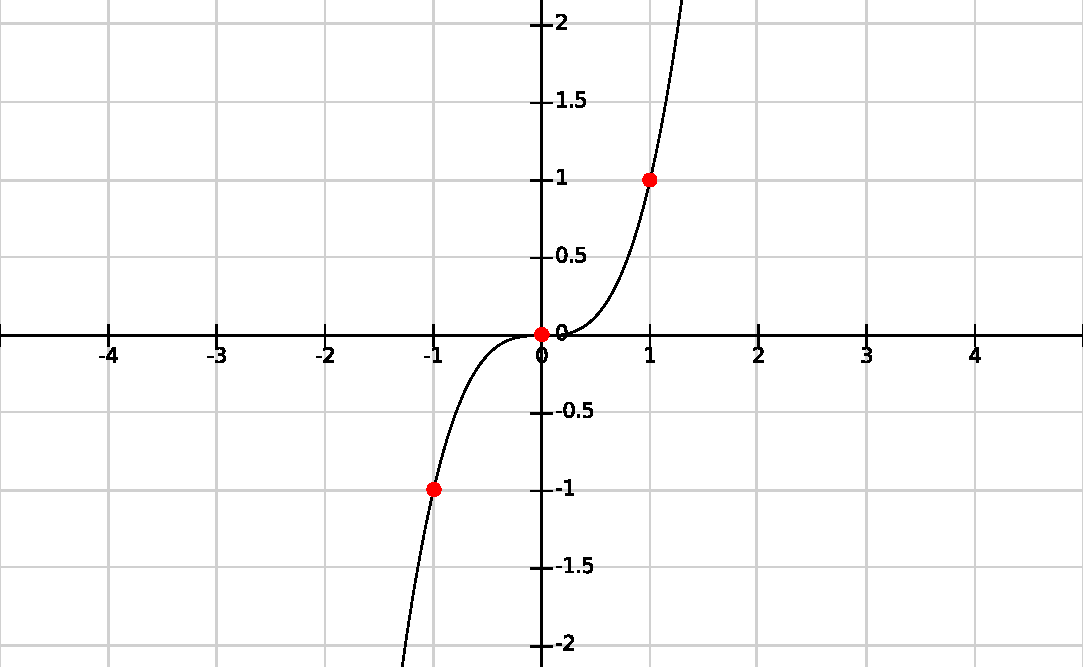
\includegraphics[width=0.4\paperwidth]{fixed_point_x_cube_withdots}
\caption{$f(x)=x^{3}$ and its fixed points, (in dashed grey, the function $y = x$)}
\label{fixed_points_x_3}
\end{figure}

An obvious property of fixed points is that $x_{fp} = f(x_{fp}) = f(f(x_{fp}))$ ...

A fixed point can be \emph{attracting} or \emph{repelling}. A fixed point is said to be attracting when when we converge toward it when iterating over $f$ in its neighborhood. Conversely, a fixed point is repelling if we diverge while doing so. A fixed point which is neither attracting nor repelling is said to be \emph{neutral}.

[[insert diagram of attractive and repelling fixed points]]

A fixed point $x_{fp}$ will be attracting if $|f'(x_{fp}| < 0$.\\
If $|f'(x_{fp}| > 0$ then the fixed point is repelling.\\
At last is $|f'(x_{fp}| = 0$ then $x_{fp}$ is neutral.


\subsection{Fixed Point with Coupled Functions}

The notion of fixed point can be extended to coupled functions.


\section{Mono-Level Methods}

\subsection{Multidisciplinary Feasible}

Multidisciplinary Feasible (MDF), is the most basic and classical MDO method. This approach ensure at each optimization step that the design is consistent as a whole, taking in account all the disciplines together (hence the name). The optimizer only use the design variables, objective functions and constraints.
Basically, MDF alternates between a MDA and a [[global]] optimization phase, ensuring the design to be globally consistent at each optimization step. At each step, the result proposed by the optimizer is used to do a full MDF whose results are used in return for the next optimization iteration.

As it is so straightforward, MDF requires no reformulation of the problem, unlike most of the others MDO methods, and in so is really easy to use. As the design is consistent at each step, the optimization process can provide a solution at any time (but it will not guarantee that the proposed solution will satisfy the constraints, as this concerns depend on the optimization technique used). However, since MDA is supposed to be costly, MDF is often considered to be quite inefficient, since it never exploits the parallelization opportunities dues to the separation of the disciplines. MDF does not provide any guarantee of convergence.

[[formulation + Diagram to illustrate the method]]


\subsubsection{Asymmetric Subspace Optimization}

Asymmetric Subspace Optimization (ASO) is a relatively recent work of Chittick and Martins\cite{Chittick:2007:B} to improve on MDF for MDO problems where some the disciplines are specifically more costly to analyze than the others. The classical illustration given is the one of high-fidelity aerostructural optimization, where the analysis of the aerodynamic is significantly more heavier than the structural analysis. An intermediate optimization phase for the structure is introduced during the MDA, in order to reduce the number of iterations needed at the global level.
This approach can lead to significant improvement over MDF in the context of disciplines with significant analysis costs. However when the analysis costs of the disciplines are comparable, this is approach is less efficient than MDF, as it introduce extraneous optimization step.

It should be noted that this approach is not mono-level as it introduces several optimizers and a hierarchical structure. [[Then why put it here and not in multilevel ?]] 

\subsection{Individual Discipline Feasible}

Individual Discipline Feasible (IDF) differs from MDF in the way that it ensure at each step consistency for each discipline separately, but not consistency between disciplines. The global consistency of the system is not ensured until convergence.
Instead of a full MDA (as in MDF), IDF alternates the optimization with independent disciplines analysis.
However, as the variables shared among the disciplines are not guaranteed to to be consistent, IDF need to introduce a reformulation of the problem where the shared variable are duplicated among the disciplines and several equality constraints need to be added to ensure the eventual consistency.

\subsection{All-at-Once}

All-at-Once (AAO) can be seen a the opposite extreme of MDF, given that it does not try to maintain consistency neither at the global or discipline level during the optimization process until convergence.
All variables are considered as design variable for the optimizer, and the analysis equations are transformed into equality constraints.
This transformation allows the analysis phase to be very quick, as we only need to evaluate the residuals of the equality constraints representing the equations.
However, the drawbacks of IDF are even more important, as AAO requires an even bigger reformulation of the problem, introducing a lot of duplicated variables and consistency  constraints to the problem. This reformulation also complicates the optimization phase.

\section{Multi-Level Methods}

\subsection{Concurrent Subspace Optimization}

Concurrent Subspace Optimization (CSSO) is one of the firsts multi-levels MDO methods. Before the optimization, the problem is decomposed in several subspaces related to the different disciplines. Each optimization iteration then start by a system analysis, followed by a series of subspaces optimization (possibly concurrently), where each optimization tries to solve the global problem by using approximate models of the rest of the system. After the subspaces optimizations, a complete MDA is done to perform a global optimization and update the approximate models.

Originally, CSSO was developed for single-objective optimization problems. However several efforts have been made to extend CSSO to multi-objectives problems.

[[From Concurrent Subspace Optimization for Aircraft System Design -  Ke-shi Zhang:
"In recent years more work (Aute \& Azarm, 2006; Huang \& Bloebaum, 2004; McAllister et al., 2000; McAllister et al., 2004; Orr \& Hajela, 2005; Parashar \& Bloebaum, 2006; Tappeta \& Renaud, 1997; Zhang et al., 2008) has focused on extending existing MDO method to handle such multi-objective MDO problems, by means of integrating a multi-objective optimization method within the MDO framework. This kind of method can be called a multi-objective MDO method.
It is an effective way to integrate multi-objective optimization method within the CSSO framework to develop the multi-objective MDO method. CSSO was extended to solve multi - objective MDO problems, including the Multi-objective Pareto CSSO (MOPCSSO) method, Aeronautics and Astronautics the Multi-objective Range CSSO (MORCSSO) method, the Multi-objective Target CSSO (MOTCSSO) method, the Multi-objective Genetic Algorithm CSSO (MOGACSSO) method and Adaptive Weighted Sum based CSSO (AWSCSSO). In MOPCSSO the Constraint method is integrated within CSSO framework (Huang \& Bloebaum, 2007). In MORCSSO and MOTCSSO the concept of designer preference is introduced (Huang \& Bloebaum, 2004). In MOGACSSO the Genetic Algorithm is combined with CSSO and in the hope of improving the computational efficiency (Parashar \& Bloebaum, 2006). In AWSCSSO the Adaptive Weighted Sum method is introduced into CSSO (Zhang et al., 2008). "]]

\subsection{Collaborative Optimization}

Collaborative Optimization (CO) \cite{Ilan:1994:MOM:887207} reformulate the problem by replacing  dependencies between disciplines by equalities constraints. This transformation allows to solve in parallel discipline-level optimizations problems. A system-level optimizer is then used to minimize the discrepancies (via the added equalities constraints), while maintaining the satisfaction of the disciplines constraints.
CO is best-suited for MDO problems with a low coupling between disciplines. The authors have argued that one advantage of CO is that it closely matches the discipline decomposition of the problem, as the scope domain-specific variables and constraints are limited to the related disciplines. Thus, the discipline optimizations can be done by domain experts  who have a strong understanding of the subproblems.

\subsubsection{ECO}

\subsection{Bilevel Integrated System Synthesis}

Bi-Level Integrated System Synthesis (BLISS) \cite{J.:1998:BIS:886310} has been developed to separate local and shared variables, in order to ease the distribution of the optimization process (be it in regard of expert teams or computational resources).
BLISS shares similarities with CSSO [[explain]]. However, local variables are assigned to the disciplines optimizations while the global variables are assigned to the global system optimization.

For each discipline optimization problem, an approximation of the global objective-functions and constraints is build using linear approximation considering only the variables of the discipline.

The optimization process cycle alternates as follow: First a system-wide analysis is done (which includes the analysis of each subsystem) and used to provide the approximate objective-functions. Then a discipline-level optimization of the objective-functions approximations, which is used for a system optimization concerning the shared variables. These results are then used by the new system analysis at the start of the next step.

\subsubsection{BLISS 2000}
[[DELETE susbusbsection ? => NOPE it is different, see Musltidisciplinary Design Optimization: A survey of Architectures:
"    A radically different formulation called BLISS-2000 was developed by Sobieski et al; . Because BLISS-2000
does not require an MDA to restore the feasibility of the design, we have separated it from the other BLISS variants
in the classification shown in Fig. 7. In fact, like other IDF-derived architectures, BLISS-2000 uses coupling variable
copies to enforce consistency at the optimum. Information exchange between the system and discipline subproblems
occurs through surrogate models of the discipline optima"
]]
   
\subsection{MDO based on Independent Subspaces}

MDO based on Independent Subspaces (MDOIS) \cite{NME:NME1380} has been developed for handling problems where the different disciplines are coupled (i.e. some outputs of one discipline are used as inputs by the others and vice versa) but they do not share any design variable or criterion.
MDOIS decomposes the system in separate subsystems, for each an optimization problem is defined, with its own design variables, objective-function and constraints. The coupling variables are considered constant for these subproblems. After each subsystem has solved its optimization problem, the new values of its variables are used in a system-wide analysis to be re-injected for the next iteration of subsystem optimization.

\subsection{Quasiseparable Subsystems Decomposition}

Quasiseparable Subsystems Decomposition (QSD) \cite{1389-4420} is another specialized method for systems which can be decomposed into subproblems which only depends on local variables and global design variable but not on values produced by others subsystems. 

[[CO/ECO, CSSO, ATC,  BLISS, EPD/IPD, MDOIS, QSD]]

\chapter{Conclusion on Optimization}

We have seen in this part how different types of optimization problems have been defined over time, depending on their topology, their complexity, their specificities.

Something worth noticing is the fact that all these types of problems are not \emph{inherently} different, but share a common structure.
Indeed, a mono-objective optimization problem is just a special case of a multi-objective problem. A multi-disciplinary problem is basically a optimization problem so complex that standard optimization techniques fail.
These distinctions where made because of the limitations of the optimization techniques, which have to choose between being applicable in the general case and being efficient.

An interesting observation concerning MDO techniques is the fact that, to evaluate their performances, they are sometimes applied to simple optimization problems, solvable by numerical optimization techniques (see for example \cite{Kroo:1994:MOM} for an application of CO to the Rosenbrock's valley problem). This observation illustrates the fact that all optimization problems share a common structure and differ only in their complexity. Of course these examples are usually only used as illustration, as MDO methods are too heavy to be interesting to use for such problems.

These conclusions raise an interesting question: could it be possible to create an optimization technique which would scale from simple optimization problems to complex ones?

In itself this statement seems to be contradicted by the intuition provided by the NFL theorems. However we have also seen how at the extreme end of complexity, the concern is not so much about finding an efficient optimization technique, but finding an efficient \emph{organization} to apply specialized optimization techniques to the different parts of the problem, while keeping a global coherence.
At this level, the actual optimization processes can be abstracted as black boxes, which are handled behind the scene by experts or automated processes.

Thus we can reformulate our question as: could it be possible to create a technique which would provide an adequate organization for each type of problem, adapted both to simple problems which need to be solved quickly and to large-scale optimization problem involving whole disciplines?

Currently, only MDO techniques could be seen as being applicable to the whole range of optimization problems, but their strict structure make them to cumbersome for for such a task.
An ideal solution for such a problem would be a method able to adapt itself to the problem at hand, in order to scale with the needs of the engineers.

The next parts of this thesis concentrate on providing such a method.



\part{A Multi-Agent System for Optimization}

\chapter{Agent-Based Modeling of an Optimization Problem}

\section{From an Optimization Problem to a Multi-Agent System}

\chapter{Simulation Rules}

\chapter{Solving Rules}

\chapter{Implementation}

\section{MAY Architecture}

To implement the MAS, we used the Make Agents Yourself (MAY) framework. MAY is a component-based framework which automatically generate an implementation of an agent architecture from a given description.

[[PROVIDE SOME REF -> ASK VICTOR]]

The Adelfe methodology proposes an abstract agent architecture (represented in \fig{[[TODO]]}), which we translated into the MAY architecture description language, SpeADL. [[As our agents only act and communicate using message-passing, we could make some simplification concerning the modeling of the communication and action capabilities.]]
All our agents use the same AMAS architecture. They are differentiated by specific implementations of the components. For example, \emph{Model} and \emph{Variable} agents will have different implementations of the \emph{Behavior} component.

For the sake of clarity, the agent architecture is separated in three views: the \emph{behavior}, \emph{communication} and \emph{monitoring} views.

\subsection{Behavior}

The \emph{behavior} view (\figurename \ref{Arch-behavior}) contains the components related to the behavior of the agent. 

\begin{figure}
\centering
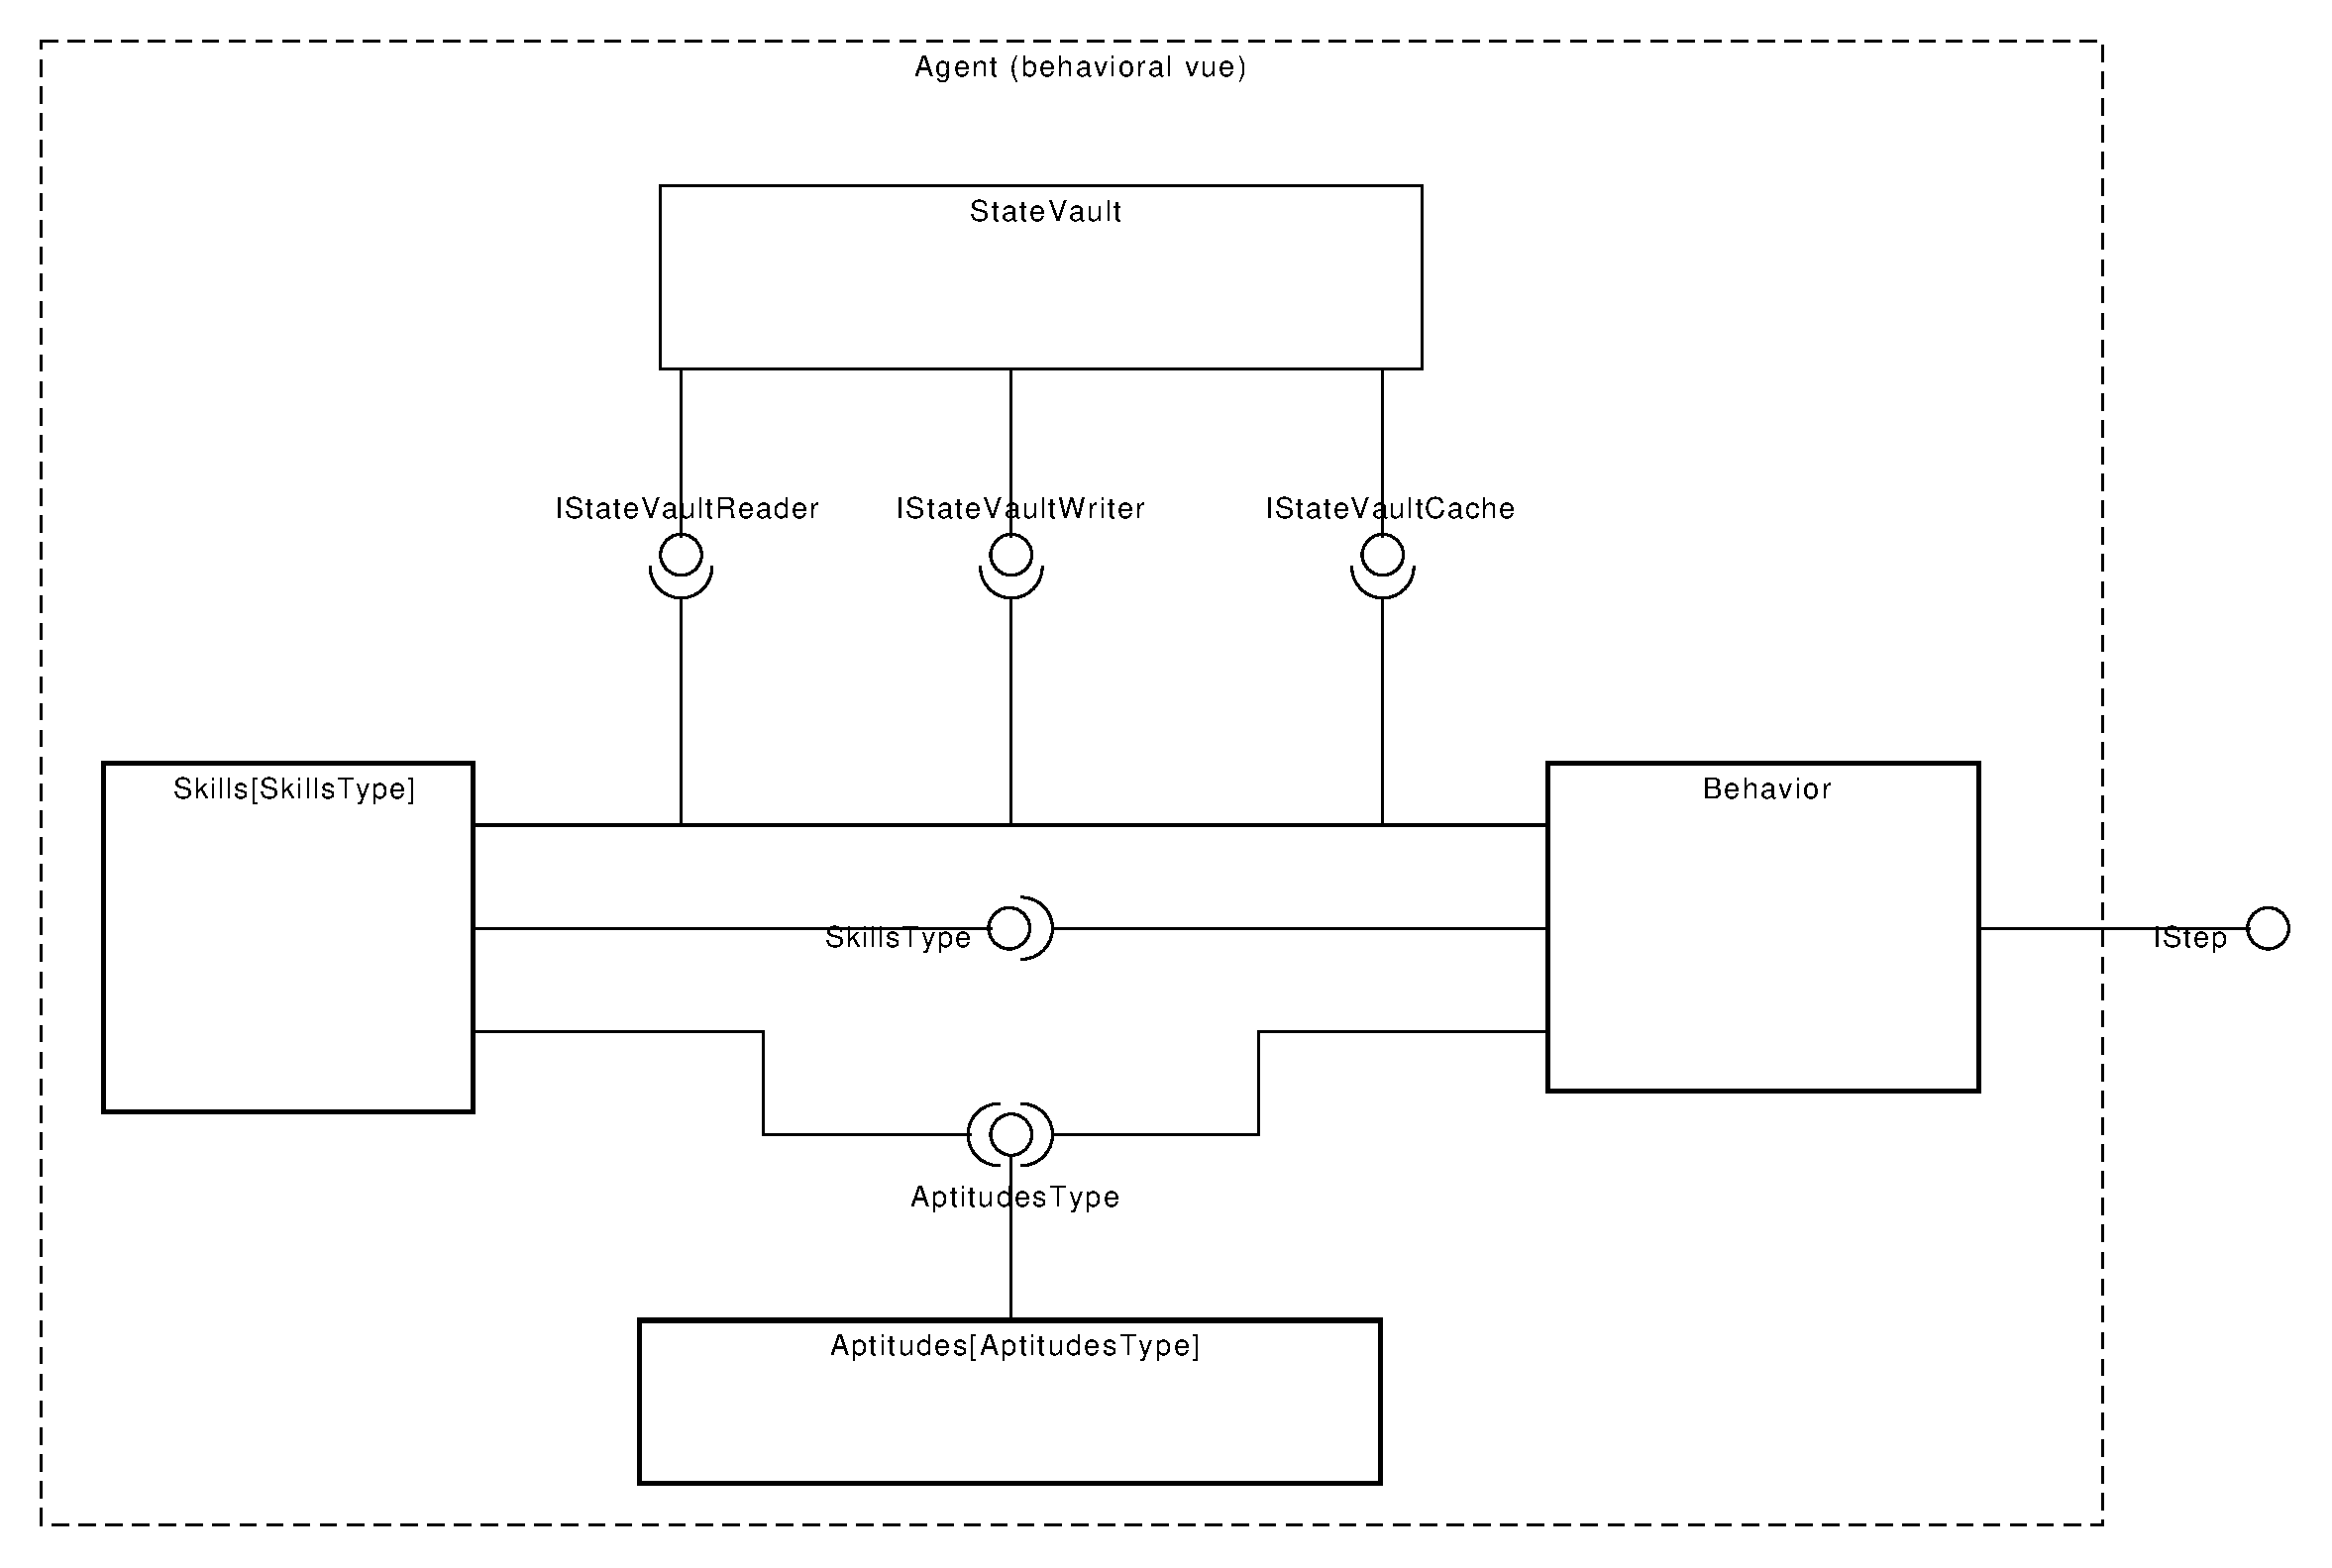
\includegraphics[width=0.6\paperwidth]{ID4CS_Speadl_behav}
\caption{Agent Architecture - Behavior view.}
\label{Arch-behavior}
\end{figure}

The \emph{Behavior} component contains the rules which dictate the behavior of the agent. This component can be seen as the [[chef d'orchestre]] of the architecture. This component exposes to the outside of the environment the \emph{Step} port, which is used to make the agent execute a step. During a step the \emph{Behavior} component executes the agent rules. These rules will in return make use of the others components of the agent.

[[DIRE QUE LES RULES ONT ETE PRESENTEES DANS UN CHAPITRE PRECEDENT]]

The \emph{State Vault} contains the state of the agent. It is used by the components which need to save and read some state variables. Centralizing all the states variables into one component provides several benefits. First it is easier to save and restore the state of the agent, as we just need to save the content of the vault. It is also simple to share some data between components, as long as these components have access to the vault. And it is easy to provide a view of the agent state by just reading the State Vault.
This approach has however several drawbacks. It adds some boilerplate code when writing code using the agent state, as we need to explicitly read the value from the vault (and possibly store it to the vault if modified). It make more difficult to track side-effects, as it is not obvious to know which component uses which value. At last there is no way to strictly enforce that components only use the State Vault for storing state values, as neither Java nor MAY can provide such guarantee.

The \emph{Skills} component contains the skills of the agents. Skills are [[skill definition]]. Each agent type has its own skills set, and skills can require to read and modify the agent state (thus the link between this component and the \emph{State Vault}).
Some skills are used directly from the \emph{Behavior} rules but some skills can also be used by others skills.
Some examples of skills are: for a \emph{Variable agent}, the capability to change its value based on the requests it received and its old value. For a model agent, the capability to translate a request it received to change one of its outputs into a set of requests to send to its inputs.

[[PARLER DU FAIT QUE LES SKILLS ONT LEUR PROPRE ARCHITECTURE ??]]

The \emph{Aptitudes} component contains the aptitudes accessible to the agents. Aptitudes are [[Aptitude definition]]. Unlike skills, aptitudes are general capabilities which do not rely on the state of the agent. Consequently, all agent types have access to the same aptitudes, and there is only one implementation of the \emph{Aptitudes} component.
Some aptitudes are used directly from the \emph{Behavior} rules but some aptitudes can also be used by skills or others aptitudes.
Some examples of aptitudes are: ordering a set of requests from the most to the least important. Make some manipulations on the exchanged values (adding, calculate the norm etc.).

\subsection{Communication}

The \emph{communication} view (\figurename \ref{Arch-comm}) presents the components related to the communication capabilities of the agent. 

\begin{figure}
\centering
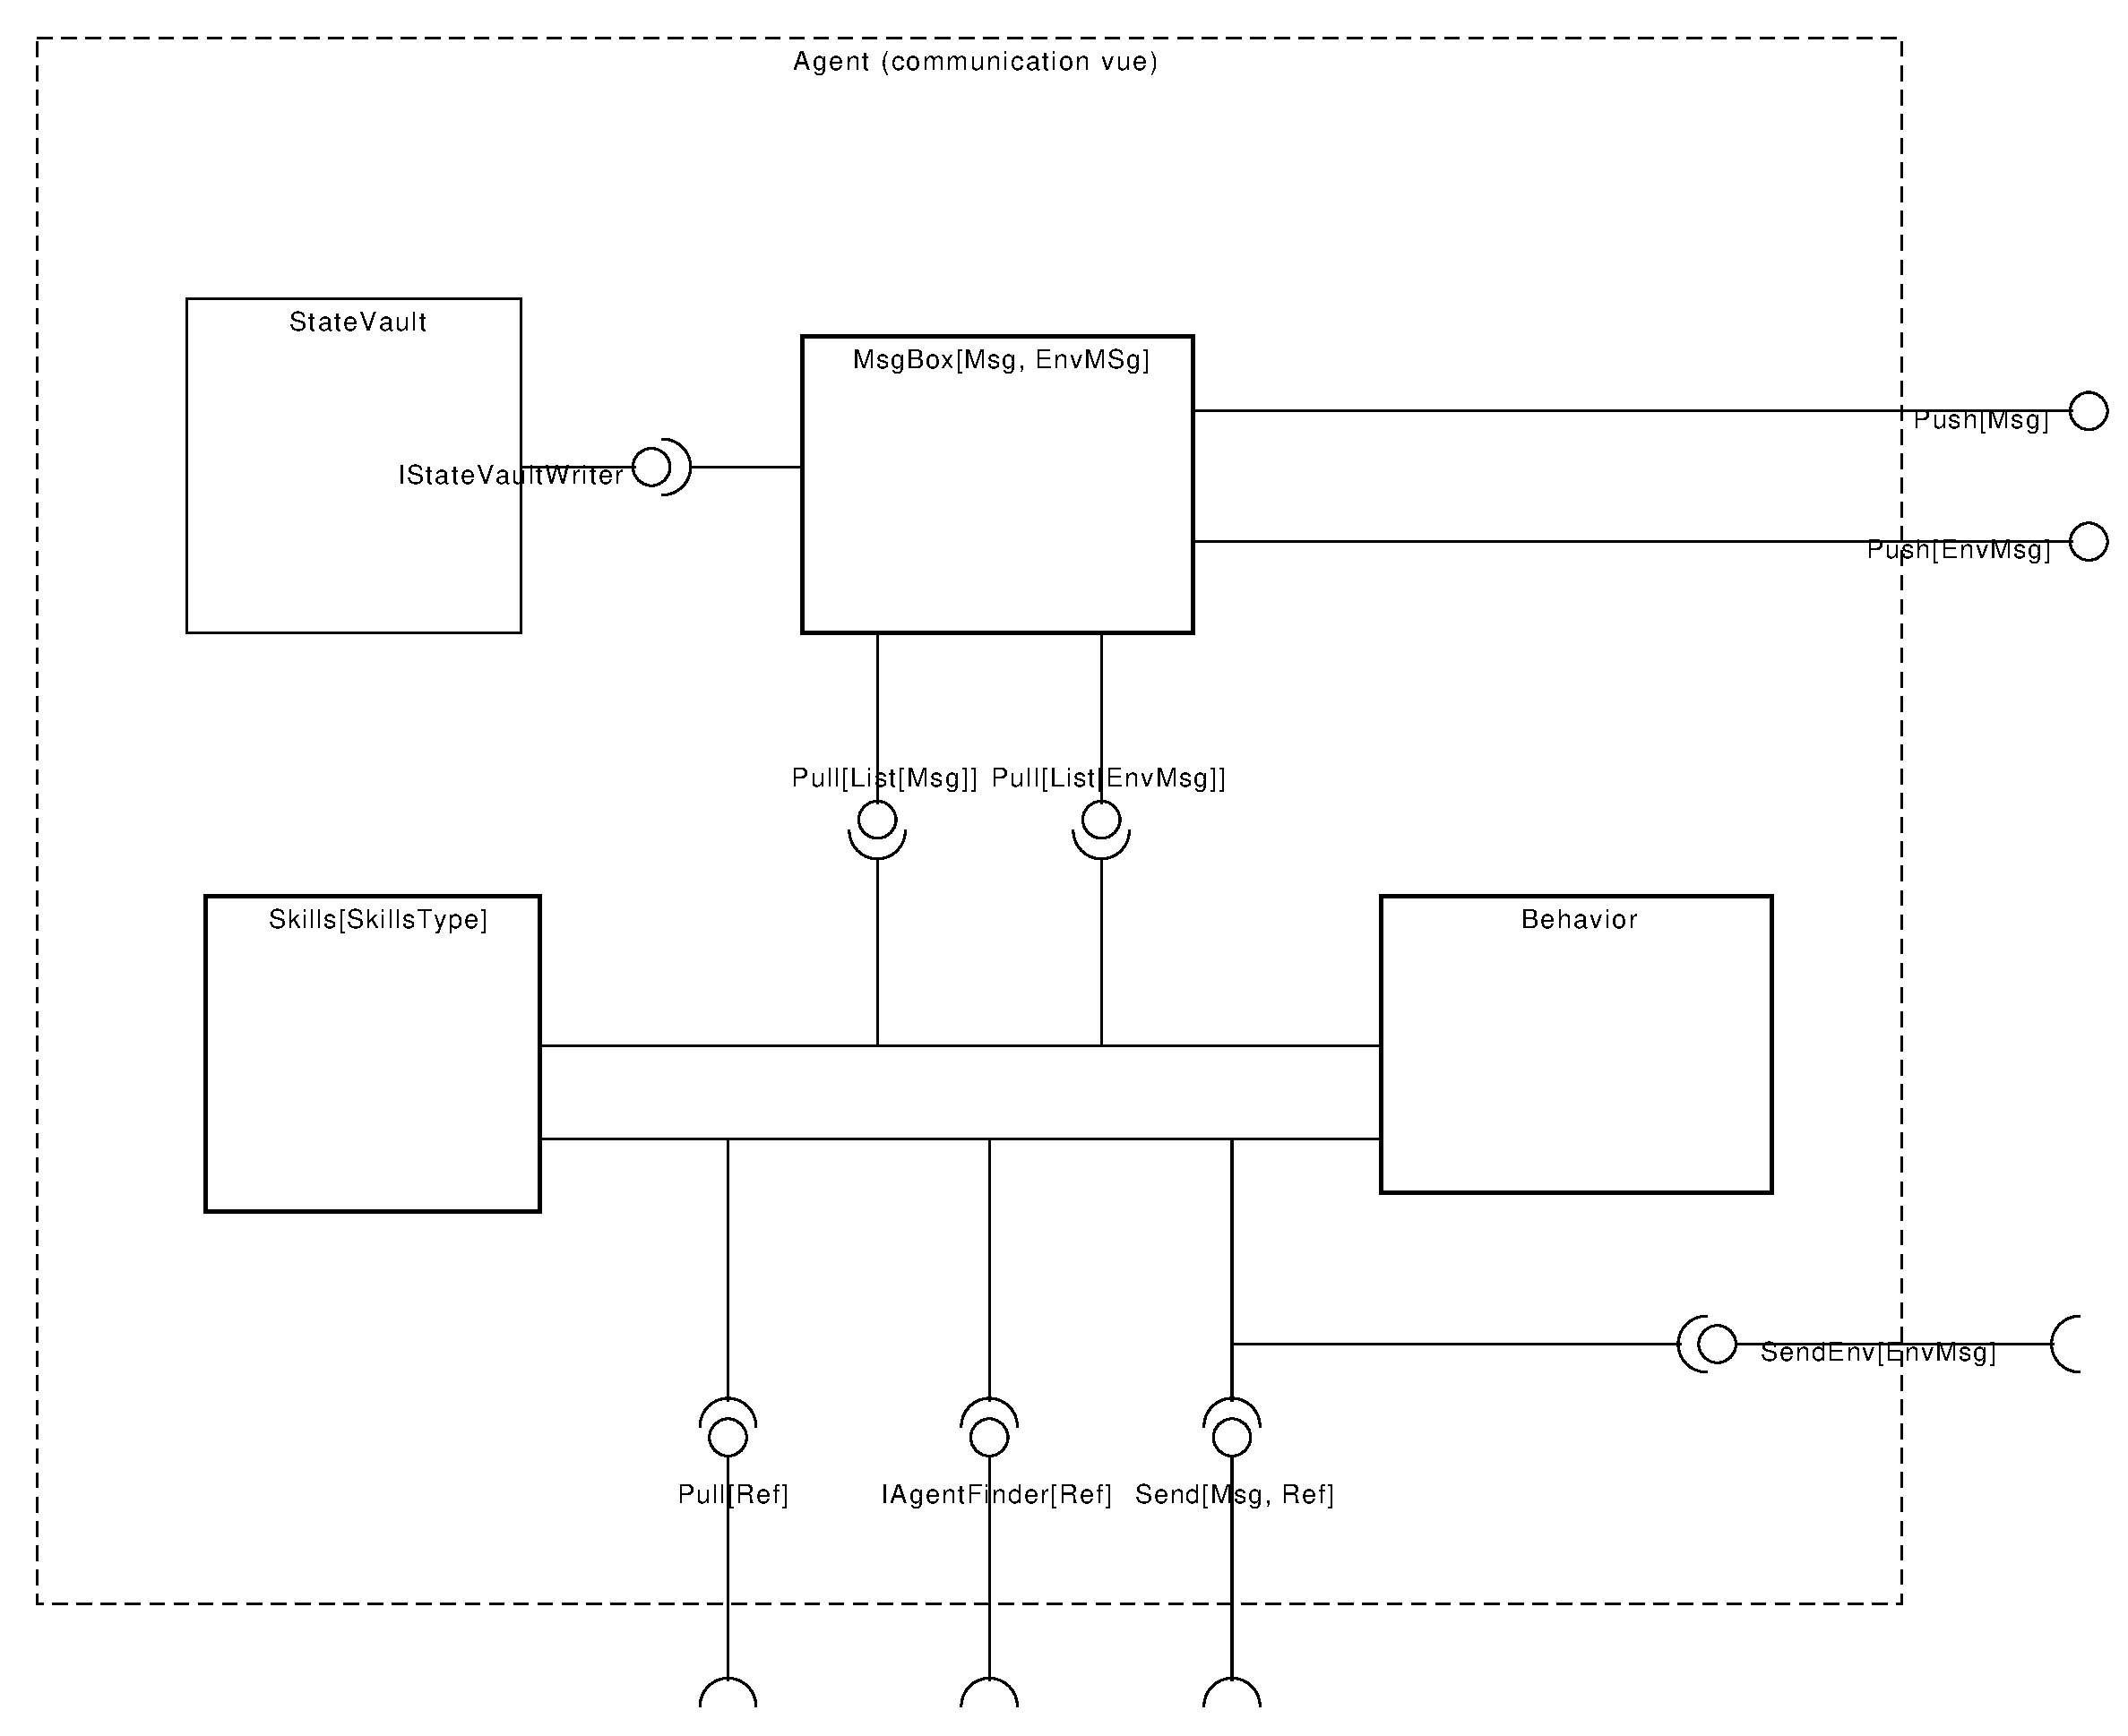
\includegraphics[width=0.6\paperwidth]{ID4CS_Speadl_comm}
\caption{Agent Architecture - Communication view.}
\label{Arch-comm}
\end{figure}

This view contains the new component \emph{Message Box}, which contains the messages sent to the agent. The \emph{Message Box} stores the messages into the \emph{State Vault} and provides a direct access to the \emph{Skills} and {Behavior} components.

This figure presents several ports which need to be provided from the environment to the agent. The environment must give an unique \emph{Reference} to the agent, which will be used by the others agent to communicate with it. The environment must also provides some ports to communicate with the others agents and outside of the system.
[[PARLER DE L'AGENT FINDER ??]]

\subsection{Monitoring}

The \emph{monitoring} view (\figurename \ref{Arch-monitor}) presents the components related to the monitoring of the agent. 

The new component introduced in this view is the \emph{Monitor}. The \emph{Monitor} provides to the environment to ports. The first port is used for external monitoring interfaces to subscribe to be informed of changes in the state of the agent. The second is used to provide informations concerning changes of a specific part of the agent. Thus, an external monitoring interface can subscribe to be notified when the state of the agent changed using the first port, and then use the second port to access to the specific informations it want to monitor.

In order to provide its capabilities, the monitor agent need to be informed by the \emph{Behavior} component before and after each step, to read and compare the monitored informations into the \emph{State Vault}.

\begin{figure}
\centering
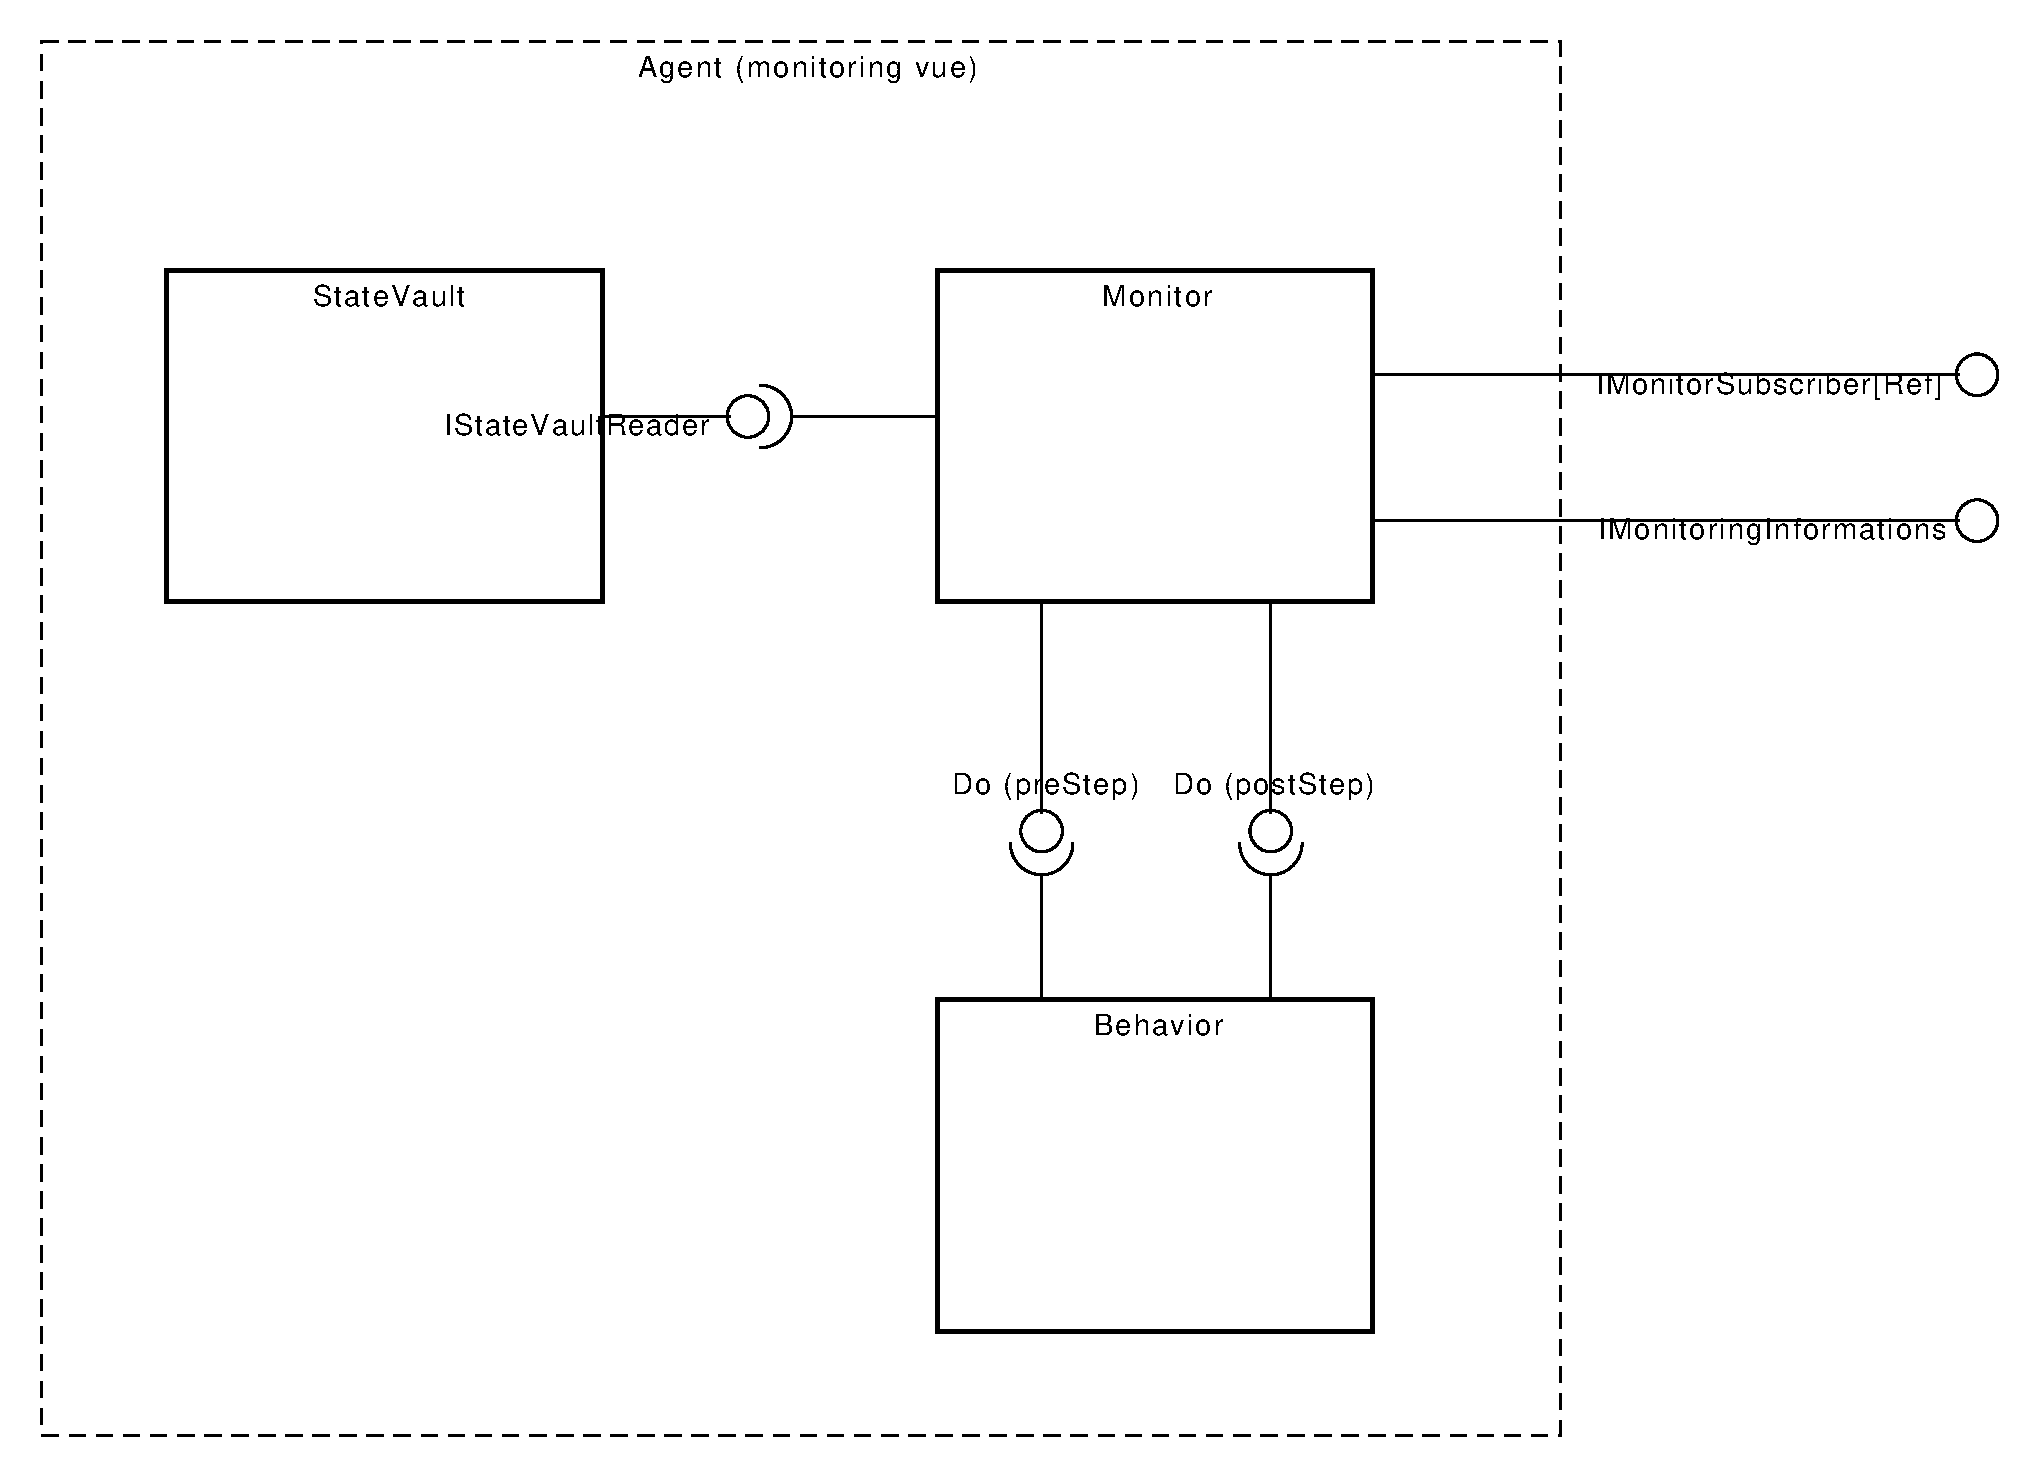
\includegraphics[width=0.6\paperwidth]{ID4CS_Speadl_monitoring}
\caption{Agent Architecture - Monitoring view.}
\label{Arch-monitor}
\end{figure}

\section{MAS Architecture}

\section{Integration into the prototype}

[[OSGI and EMF]]

\chapter{Analysis - Collective Solving Patterns}

%%%%%%%%%%%%%%%%%%%

\Conclusion{Conclusion}
%\Conclusion{Conclusion and Perspectives}

In this thesis we identified a severe limitation of current continuous optimization methods regarding the handling of complex continuation problem. These problems are usually  too complex to be solved by classical optimization methods, because of multiple factors: the interdependencies of their components, their heavy computational cost, their nonlinearities \emph{etc.}. Because of this reason, specific methods have been developed to distribute the optimization process. However these methods are often difficult to put in practice and cumbersome, not suiting the need of a flexible and iterative process often associated with such problems.

We presented in this work a \emph{new approach for solving complex continuous problems using an adaptive multi-agent system}. This system, designed following the AMAS theory, proposes a decentralized way to automatically distribute the optimization process among the agents. This system is build upon a \emph{general continuous problem modeling we named NDMO}, which transform the optimization problem into an entities graph. This transformation is, once more, fully automatic, and does not require any simplification, modification or reformulation of the original problem. While our system is the first instance of MAS using this modeling, this graph representation is generic and can be re-used as a base to propose other comparable systems.\\
Following the AMAS theory, we kept the agent perceptions and capabilities at a local level, allowing them to communicate and interact only with their immediate neighbors. Doing so, we are able to handle the problems complexity, as each agent keeps a local point-of-view. In order to maintain a global consistency, the agents exchange inform and request messages that are propagated into the system.



%%%%%%%%%%%%%%%%%%%

\appendix
\Partie{Annexes}

%\chapter{Une annexe}

%%%%%%%%%%%%%%%%%%%

\bibliographystyle{plainnat-fr}
%\nocite{*} %for to include all bibtex, even non-cited articles
\Bibliographie{StateoftheArt/SoA}

%%%%%%%%%%%%%%%%%%%

\ListeFigures{Figures List}
\ListeTables{Tables List}

\end{document}